\documentclass[conference]{IEEEtran}

% correct bad hyphenation here
\hyphenation{op-tical net-works semi-conduc-tor}
\usepackage{graphicx}
\usepackage[square, numbers, comma, sort&compress]{natbib}
\usepackage{verbatim} 
\usepackage{vector}
\usepackage{amsthm}
\usepackage{array}
\usepackage{tabularx}
\usepackage{multirow}
\usepackage{fixltx2e}
\usepackage[english]{babel}
\usepackage{amsmath}
\usepackage{todonotes}
\usepackage[]{algorithm2e}
\usepackage{pgfplots}
\usepackage[font={small,it}]{caption}
\usepackage{url}
\usepackage{pdfpages}

\begin{document}
\title{An Efficient Approach for Mining Frequent Patterns over Uncertain Data Stream}

\author{
    \IEEEauthorblockN{Md. Badi-Uz-Zaman Shajib\IEEEauthorrefmark{1}, Md. Samiullah\IEEEauthorrefmark{1}, Chowdhury Farhan Ahmed\IEEEauthorrefmark{1}, Carson Kai-Sang Leung\IEEEauthorrefmark{2}}
    \IEEEauthorblockA{\IEEEauthorrefmark{1}Department of Computer Science \& Engineering, University of Dhaka, Bangladesh
    \\mbzshajib@gmail.com, samiullah@cse.univdhaka.edu, farhan@du.ac.bd}
    \IEEEauthorblockA{\IEEEauthorrefmark{3}Department of Computer Science University of Manitoba, Canada
    \\kleung@cs.manitoba.ca}
}

% make the title area
\maketitle

\begin{abstract}
Knowledge discovery in big data is one of most interesting topic in state-of-the-art research where frequent patterns finding is a major task. With the rapid growth of modern technology, huge amount of data is flowing all over the world and incoming stream of data is not always accurate and precise. Properties of data stream changes every time with the change of interest of people that is making data dynamic. Due to the uncertainty and dynamic properties of data, it becomes a great challenge to find the appropriate and efficient approach to ensure the efficient usage of available resources. In the existing approaches, there is a trade-off between optimization (allowing false data in final result) and correctness (exact calculation/minimum resource usage). Moreover, most of them cannot handle the dynamic, stream databases. In this paper, we have proposed a new memory efficient data structure, US-tree (Uncertain Stream-tree) that stores most recent meta-information and a probabilistic, sliding window based efficient approach for handling uncertain data stream. A comprehensive performance analysis shows that our approach is scalable, correct and efficient in comparison with the recent related approaches.
\end{abstract}

\begin{IEEEkeywords}
Data Mining, Frequent Pattern Mining, Uncertain pattern, Data Stream, Sliding Window.
\end{IEEEkeywords}

\IEEEpeerreviewmaketitle

\section{Introduction}

Knowledge Discovery in Databases (KDD) has been created to identify efficient, helpful, functional and valuable information from extreme large databases and to use extracted valuable information in different applications, automated analysis, solution business and research work. In recent years, with the increase of modern technologies and huge use of internet, a lot of data is being produced. To mine interesting patterns from static database ~\cite{DBLP:conf/vldb/AgrawalS94}, ~\cite{DBLP:journals/datamine/HanPYM04} have been proposed.

Data uncertainty is an inherent property in various applications due to reasons such as hardware fault, uncertainty of incidents, outdated sources or imprecise/incorrect measurement. Data is constantly growing in volume, variety, velocity and uncertainty. On the WWW, data from sensors like GPS, weather detection machines, within enterprises both in their structured and unstructured sources, biological data, meteorological trends, of the medical behavior of living organisms data, human behavior, are the example of uncertain data. To solve finding interesting patterns from uncertain data, several approaches have been proposed ~\cite{DBLP:journals/tkde/ZhaoYN14}, ~\cite{DBLP:conf/kdd/AggarwalLWW09}, ~\cite{DBLP:conf/pakdd/LeungT13}, ~\cite{DBLP:conf/dasfaa/LeungT12}.

In the modern age, there are much more instruments like smart-phones, smart-gears (e.g. smart watch, smart glass) those have many more sensors which are collecting data each and every micro second which are imprecise or incorrect like - a temperature sensor gives some information like current temperature is 40 degree, with 5\%-10\% error. For stream data mining ~\cite{DBLP:conf/icdm/LeungK06}, ~\cite{DBLP:journals/vldb/CormodeH10} have been proposed. But none of them can handle uncertain stream data.

For uncertain stream SUF-growth ~\cite{DBLP:conf/icde/LeungH09} has been proposed. This exact algorithm has resolved the false positive and false negative generation but the constructed tree structure is like UF-growth ~\cite{DBLP:conf/kdd/GadeWK04} that suffers much as the data structure (tree) SUF-growth ~\cite{DBLP:conf/icde/LeungH09} uses to keep information is not compact which affects in the mining process and degrades performance. Hence, we have proposed a probabilistic sliding window based efficient and optimized approach for handling uncertain data stream.
Our key contributions of this paper are listed below:
\begin{itemize}
  \item We have introduced a prefix value, \emph{U\textsuperscript{cap}} for each item in a transaction which always maintains upper bound of probability. That helps us to make compact pattern tree construction.
  \item A new data-structure \emph{US-tree}, that is very much compact and very memory efficient and follow the partial downward closure property.
  \item A new mining algorithm \emph{USFP-growth} algorithm, that will reduce mining time surprisingly.
  \item Propose runtime, memory efficient and scalable approach and will have wide range of applicable area.
  \end{itemize}
  
An outline of rest of the sections is: Section \ref{Related_work} describes the necessary related works and existing approaches. Section \ref{proposedWork} provides the details of our proposed approach with required analysis. Experimental results in detail with comparison and analysis are given in Section \ref{Experiment}. Section \ref{Conclusion} ends the thesis with a brief conclusion and future scopes.

\section{Related Work}\label{Related_work}
\begin{table}
\centering

\begin{tabular}{|c|c|c|c|c|c|}
\hline
	Batch No& Transaction No & \multicolumn{4}{c|}{Items in Transaction} \\ \hline \hline
	\multirow{3}{*}{Batch 1}	&	T\textsubscript{1} & a(0.9) & c(0.54) & d(0.45) & e(0.18)		\\
								&	T\textsubscript{2} & a(0.9) & b(0.36) & e(0.09) & --			\\
								&	T\textsubscript{3} & a(0.2) & c(0.18) & d(0.63) & --			\\\hline
	\multirow{3}{*}{Batch 2}	&	T\textsubscript{4} & b(0.3) & c(0.27) & --  	& --			\\
								&	T\textsubscript{5} & a(0.1) & b(0.03) & c(0.27) & --  			\\
								&	T\textsubscript{6} & a(0.9) & e(0.27) & --	    & --  			\\\hline
	\multirow{3}{*}{Batch 3}	&	T\textsubscript{7} & a(0.1) & d(0.06) & e(0.12) & --			\\
								&	T\textsubscript{8} & a(0.1) & c(0.02) & f(0.12) & --   			\\
								&	T\textsubscript{9} & c(0.2) & d(0.09) & f(0.54) & --   			\\\hline
								
	\multirow{3}{*}{Batch 4}	&	T\textsubscript{10} &  --  &  --  &  --  & --    				\\
								&	T\textsubscript{11} &  --  &  --  &  --  & --    				\\
								&	T\textsubscript{12} &  --  &  --  &  --  & --    				\\\hline
	\end{tabular}
\caption{Example of Uncertain Stream Transaction (divided into batches and windows)}
\label{table:prefix_assigned}
\end{table}

Many algorithms have been developed for finding frequent item-sets from uncertain databases. Among them, some are Apriori ~\cite{DBLP:conf/vldb/AgrawalS94} like approach and others are FP-growth ~\cite{DBLP:journals/datamine/HanPYM04} like approach. U-Apriori ~\cite{DBLP:journals/tkde/ZhaoYN14} was proposed to mine uncertain frequent pattern that is Apriori-like candidate generation and test-based approach. UF-growth ~\cite{DBLP:conf/kdd/GadeWK04}, UFP-growth ~\cite{DBLP:conf/kdd/AggarwalLWW09} was proposed to mine frequent patterns from uncertain data but the generated tree is not compact. CUF-growth ~\cite{DBLP:conf/dasfaa/LeungT12}, CUF-growth\textsuperscript{*} ~\cite{DBLP:conf/dasfaa/LeungT12}, PUF-growth ~\cite{DBLP:conf/pakdd/LeungT13} was proposed later for mining uncertain data but they produce false positives as they work with probabilistic uncertainty modeling. All of them are unable to mine stream of uncertain data. UF-stream ~\cite{DBLP:conf/icde/LeungH09} and SUF-growth ~\cite{DBLP:conf/icde/LeungH09} proposed to mine uncertain frequent pattern from stream. UF-stream ~\cite{DBLP:conf/icde/LeungH09} suffers from both false positives and false negatives. 

The SUF-growth ~\cite{DBLP:conf/icde/LeungH09} is an exact mining algorithm that has resolved the false positive and false negative generation but the constructed tree structure is like UF-growth ~\cite{DBLP:conf/kdd/GadeWK04} that suffers much because the data structure (tree) SUF-growth ~\cite{DBLP:conf/icde/LeungH09} use is not compact. Before elaborate discussion of SUF-growth ~\cite{DBLP:conf/icde/LeungH09}, we have provided a brief discussion on the background of uncertain stream mining approaches.

UF-streaming ~\cite{DBLP:conf/icde/LeungH09} was proposed to mine frequent item from uncertain stream data. This is a sliding window-based approach, that capture most recent data. It has divided the transaction stream data in several batches, each batch is inserted into the tree structure that is UF-tree ~\cite{DBLP:conf/kdd/GadeWK04} and mine each tree using UF-growth ~\cite{DBLP:conf/kdd/GadeWK04} and put all the frequent patterns found in a UF-stream structure. For avoiding false negative, it uses a value \emph{preMinSup} less than minimum support (0 $<$ \emph{preMinSup} $<$ minimum support). Then until the window is completed, the frequent item-set is put into UF-stream tree structure. This has addressed the problems of stream uncertain data mining, but it suffers from some problems like : Unnecessary mining of each batch. As an example, say, window size is 3 and batch size is 2. If one wants the mining result at window 50 then in this approach it is needed to mine each of 1 to 50 batches for getting the result.

SUF-growth ~\cite{DBLP:conf/icde/LeungH09} addressed the limitations exist in UF-streaming ~\cite{DBLP:conf/icde/LeungH09} and outperformed it by avoiding the aforementioned potential problems for mining frequent item-set from streams of uncertain data. SUF-growth is an exact algorithm. It means SUF-growth returns only truly frequent item-set but UF-streaming returns both true and false frequent item-set. This algorithm does not need UF-stream structure to store the mined item-sets. It requires transaction databases in memory resident for assumed better performance. Instead of this it uses delayed mode for mining. As a result, unnecessary computation could be reduced and unnecessary mining is avoided.
%
%        \begin{figure*}[tb]
%        \centering
%            
\includegraphics[width=\textwidth]{visio/SUF}
%        \caption{SUF-growth ~\cite{DBLP:conf/icde/LeungH09} tree construction}%%%%%%%%%%%%%%%
%        \label{figure:suf_simulation}
%        \end{figure*}

For example, for the transaction database of Table-\ref{table:prefix_assigned}, the SUF-tree is in Figure-\ref{figure:suf_simulation}. The figure shows the construction of the SUF-tree step-by-step. As the suf tree is based on UF-tree construction approach, the node sharing is very rare. From Figure-\ref{figure:suf_simulation}, it is clearly visible that the node sharing is not that much impressive as the node should be shared if the two same item has same existential probability and in real life scenario this sharing is very rare. For this reason \emph{a(0.9)} in \emph{T\textsubscript{1}} and \emph{a(0.2)} in \emph{T\textsubscript{3}} did not share single node and the tree compactness could not be accomplished. 

Although the SUF-growth has resolved some limitations of UF-streaming ~\cite{DBLP:conf/icde/LeungH09}, some limitations still exist. The tree structure that it uses is UF-tree ~\cite{DBLP:conf/kdd/GadeWK04} structure which suffers from compactness. So SUF-growth tree also inherits this limitation, tree construction cost will be much more (both running time and memory) as the transaction grows, mining algorithm it uses is FP-growth like approach that generates a huge candidate sub-pattern tree that costs much in the mining time. It increased mining cost (both running time and memory).
\section{Our Proposed Approach}\label{proposedWork}
For stream property, we will always lose data after data stream has flown away. To deal with this, we proposed a sliding window based approach, where we keep the most recent information. For uncertain data stream, each item in different transaction has different existential probability, it becomes very difficult to merge (share) these nodes in the tree. This uncertainty property of items makes the tree unmanageable and large. We have proposed a new \emph{U\textsuperscript{cap}} value for each item that helps to share a single node when constructing the tree which we named as \emph{US-tree}. Our proposed tree \emph{US-tree} is very compact and very efficient for later mining. Later, we have described an approach for mining the \emph{US-tree}, named \emph{USFP-growth}, which is \emph{FP-growth} like approach. After that a method, for filtering and removing false positives generated by our approach in the most probable candidate frequent patterns, is proposed.

%\begin{figure*}[tb]
%  \centering
%	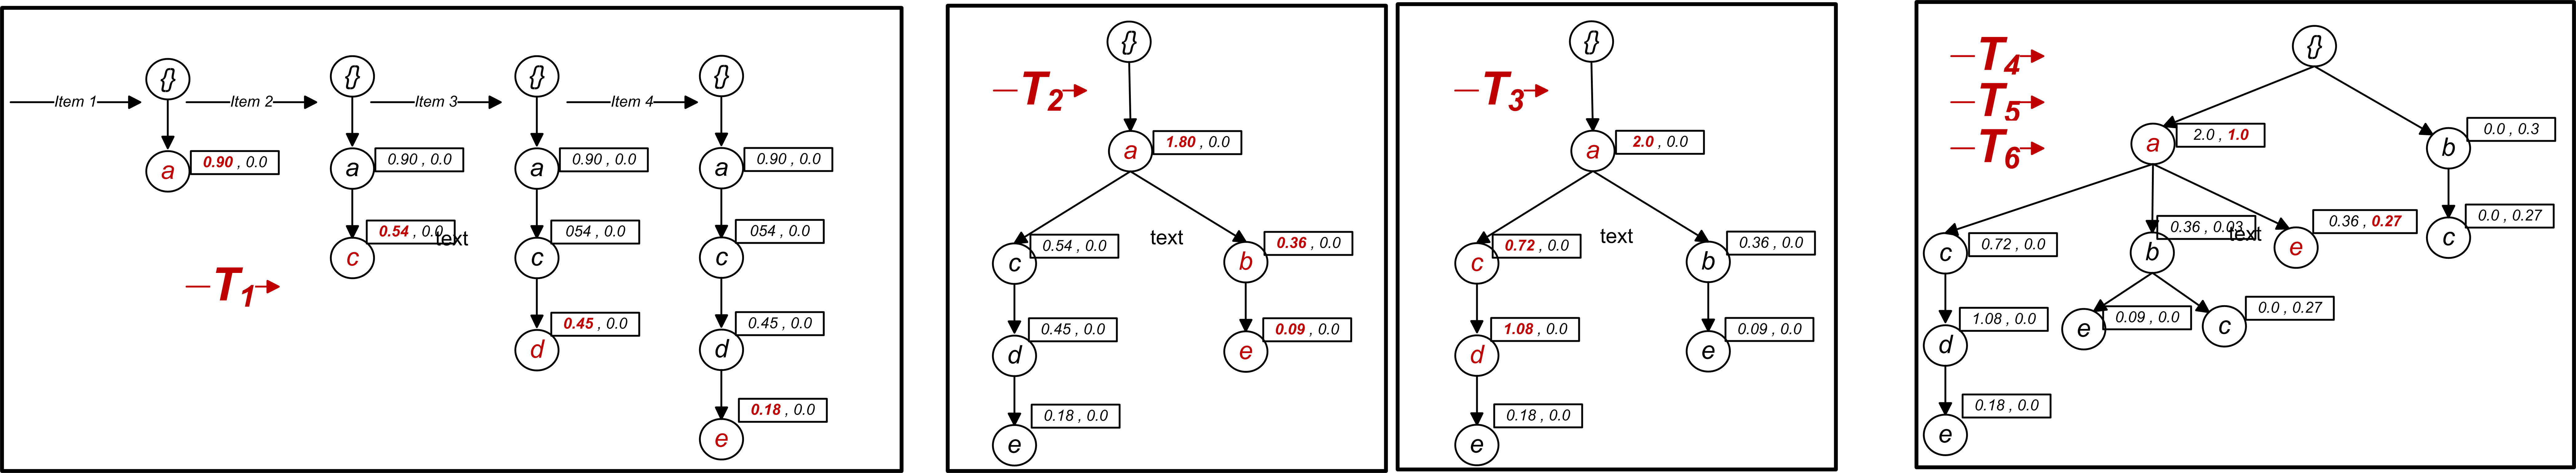
\includegraphics[width=\textwidth]{visio/sim_1_6}  
%	\caption{Constructing US-tree}%%%%%%%%%%%%%%%%%
%	\label{figure:t1_6}
%\end{figure*}
%
%\begin{figure*}[tb]
%  \centering
%	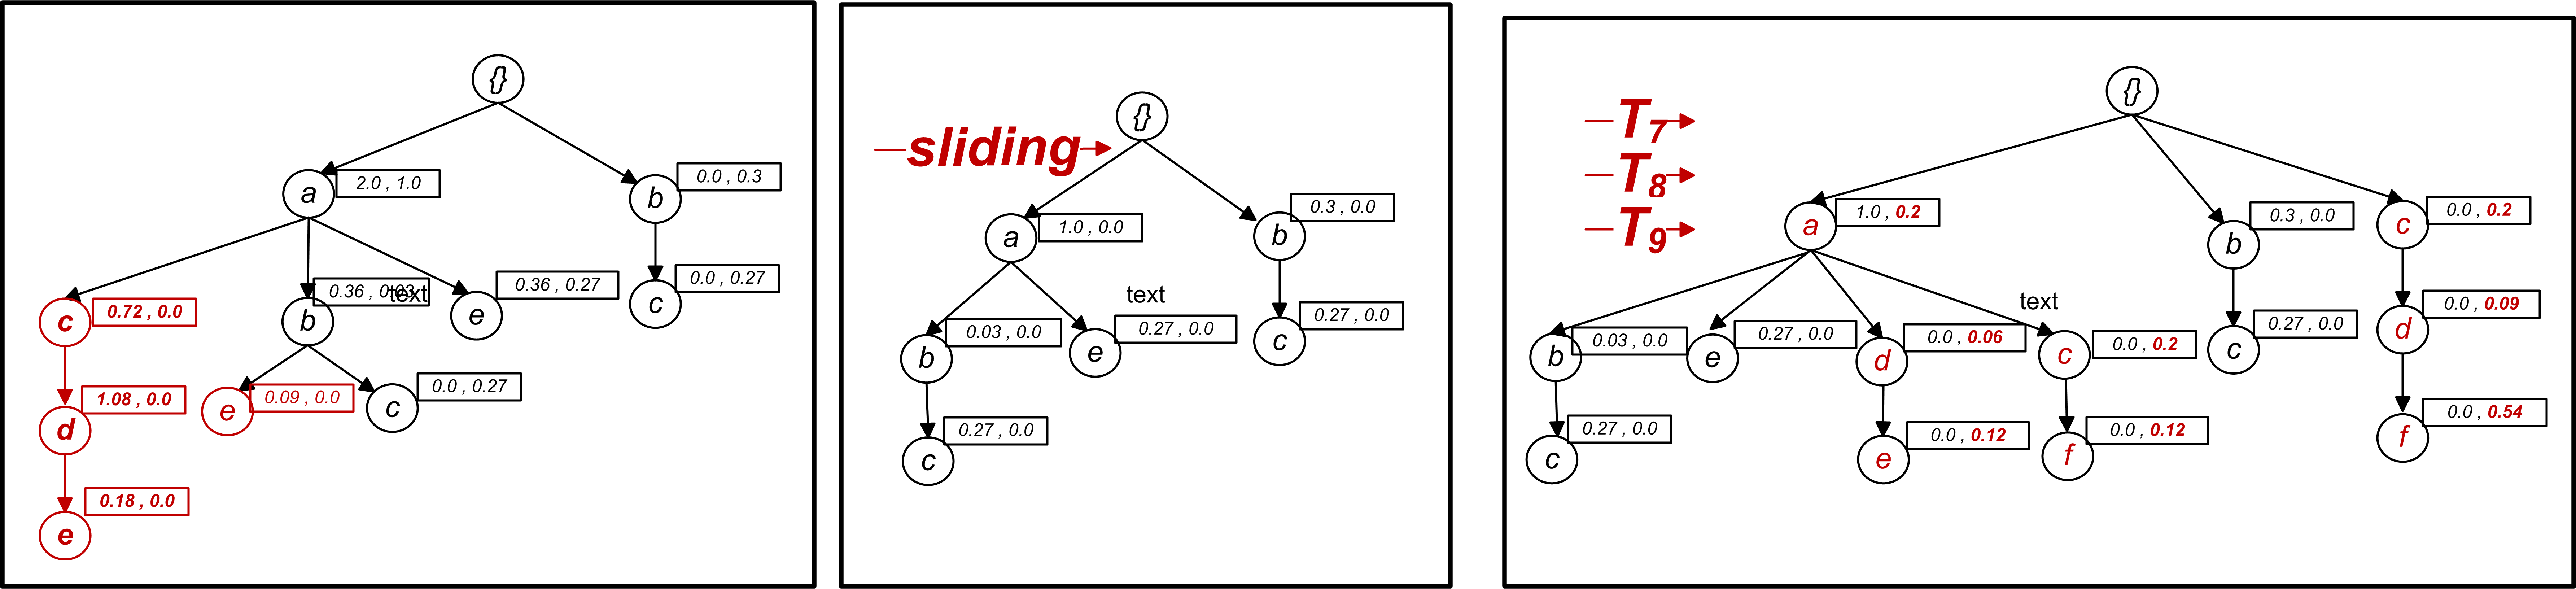
\includegraphics[width=\textwidth]{visio/sim_06_slide_789}  
%	\caption{Updating US-tree with new sliding window}%%%%%%%%%%%%%%%%
%	\label{figure:t7_9}
%\end{figure*}


\begin{figure*}[t]
    \begin{minipage}{0.5\linewidth}
        \centering
  		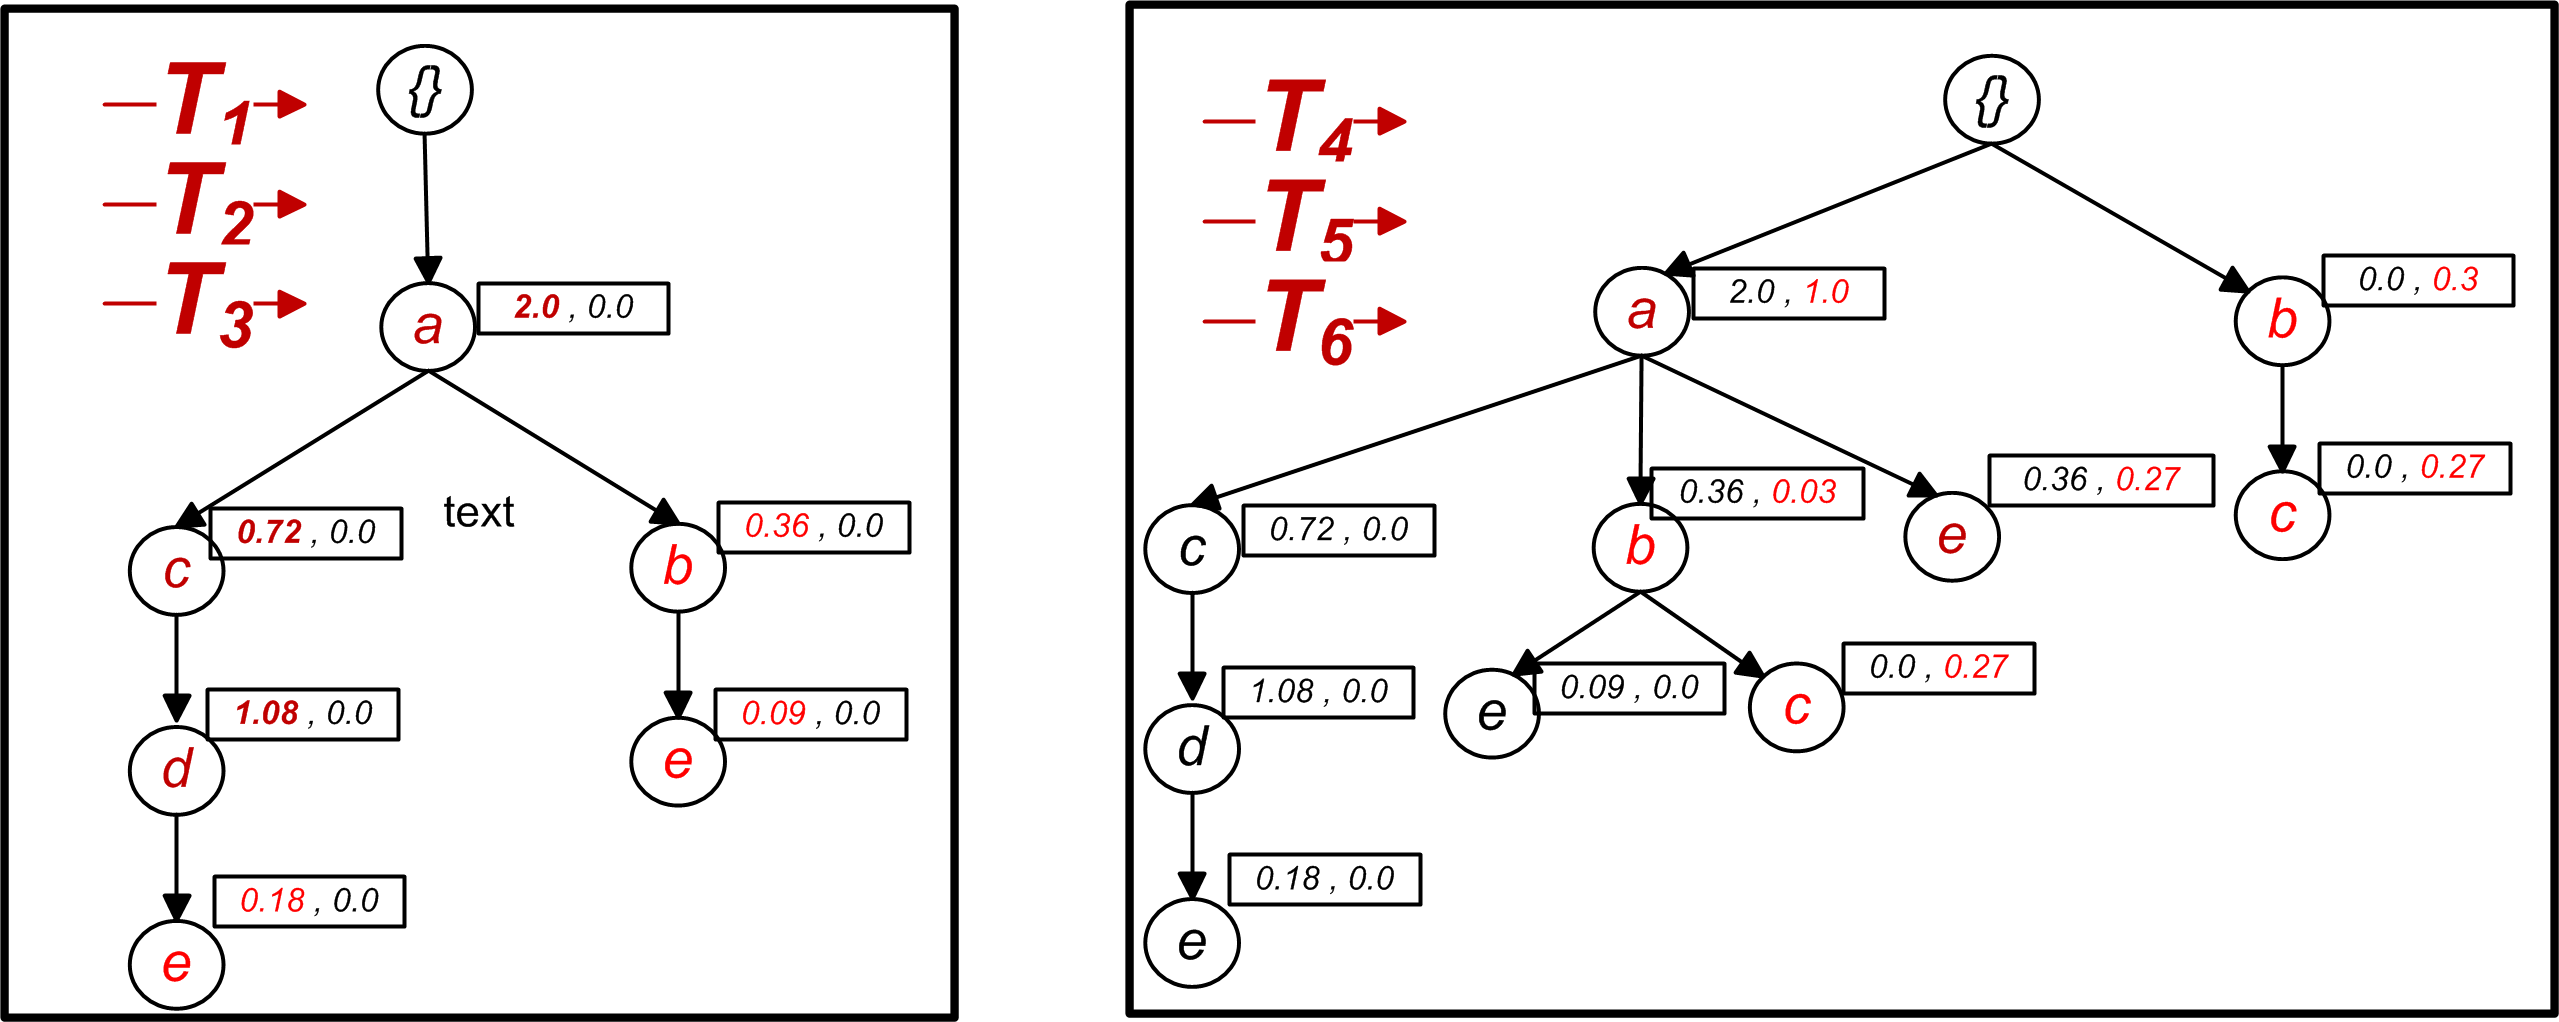
\includegraphics[width=.9\textwidth]{visio/sim_1_6_V2}
  		\caption{Constructing US-tree}
  		\label{figure:t1_6}
    \end{minipage}%	
    \begin{minipage}{0.5\linewidth}
         \centering
  		 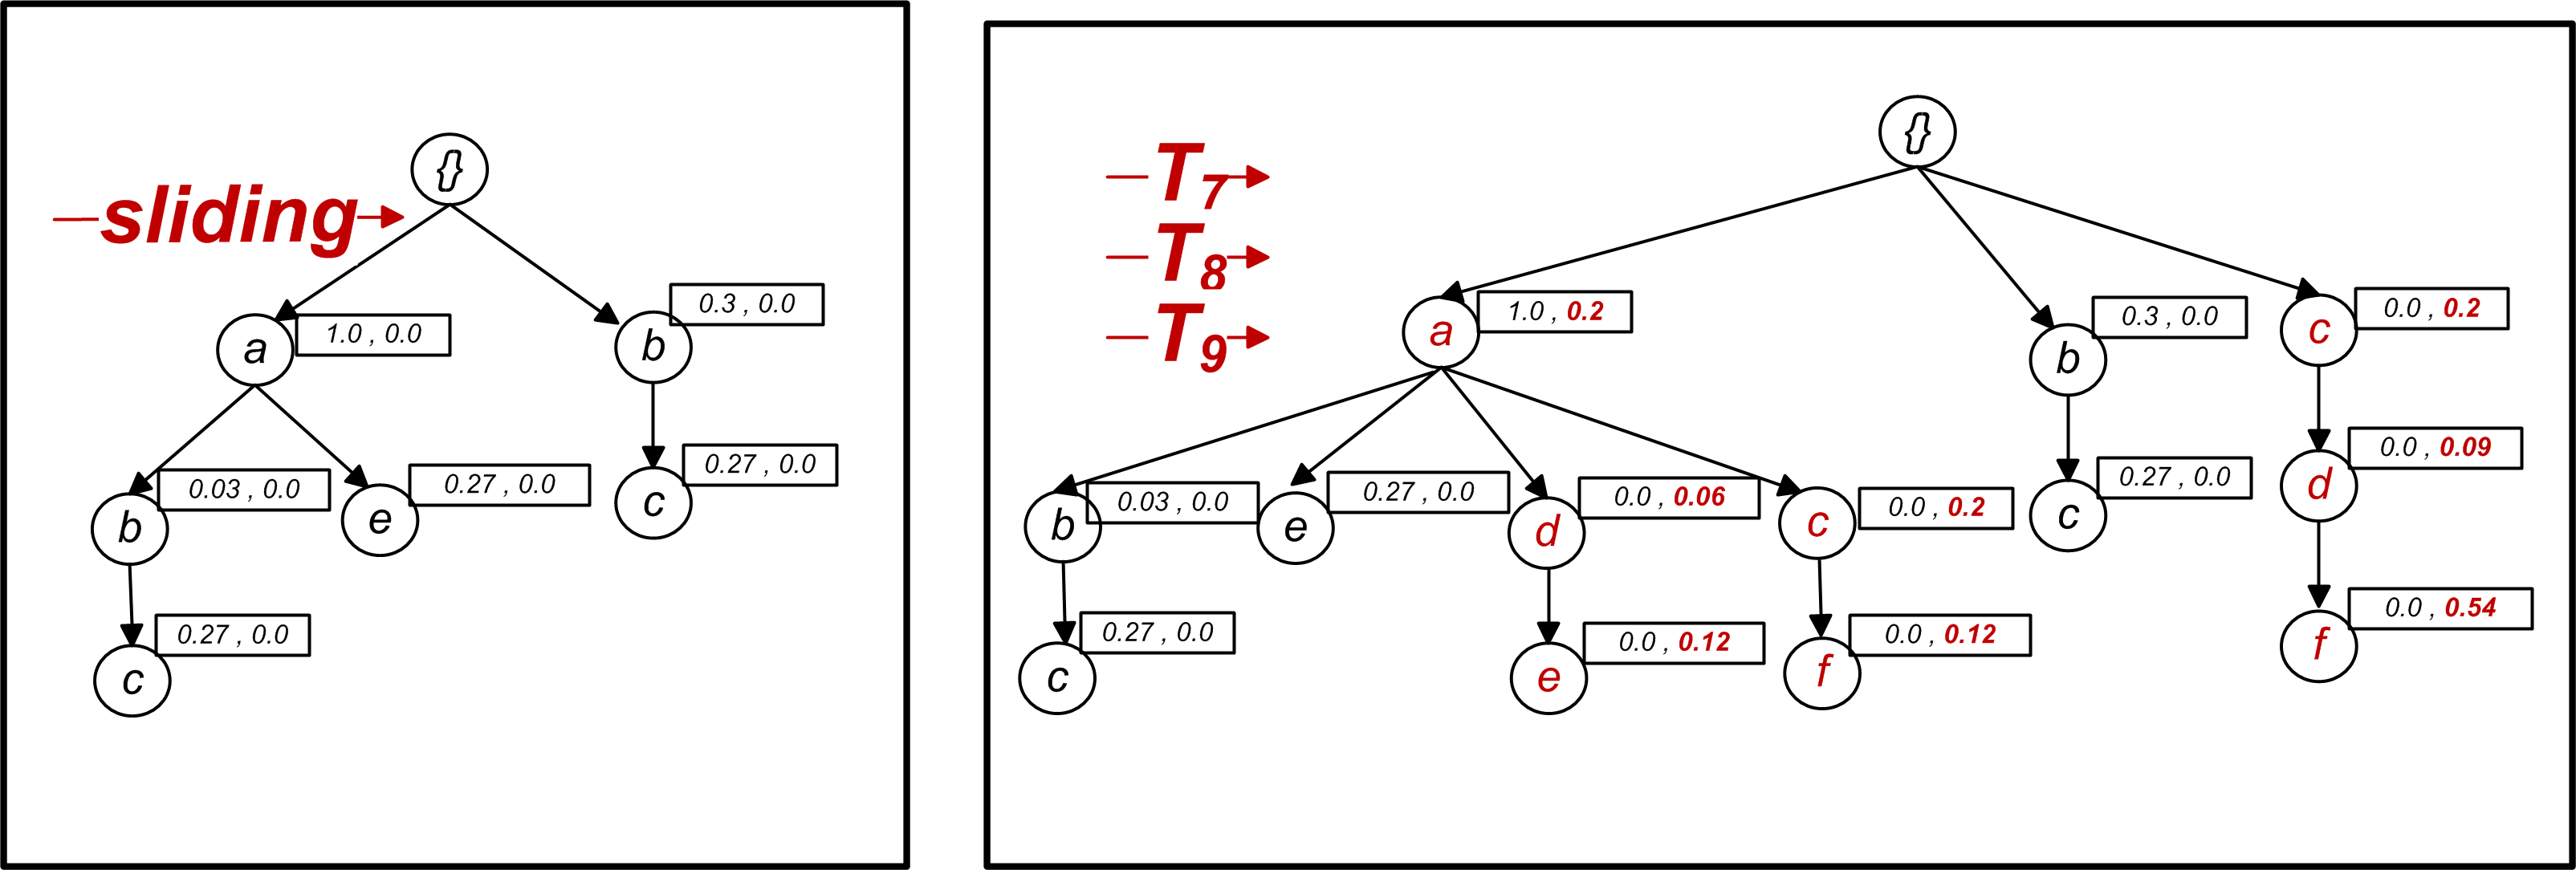
\includegraphics[width=.9\textwidth]{visio/sim_06_slide_789_V2}
  		 \caption{Updating US-tree with new sliding window}
  		 \label{figure:t7_9}
    \end{minipage}	
\end{figure*}


\subsubsection{Preliminaries}
\emph{U\textsuperscript{cap}:}
    The following equation is for \emph{U\textsuperscript{cap}} calculation.
	{\footnotesize
    \begin{equation}\label{equation:cap}
	\text{\emph{U\textsuperscript{cap}}}(X_r) =\begin{cases}
				P(X_1), & \text{if $ h = 1$}\\
				P(X_r)*M, & \text{if $ h > 1$}
             
		\end{cases}
where,\\ M=max_{1\leq q\leq h}P(X_q)
\end{equation}}

For the transaction \emph{DB} in Table-\ref{table:prefix_assigned}, for \emph{T\textsubscript{1}}, \emph{U\textsuperscript{cap}} of \emph{$a$(0.9)} is $0.9$ as $a$ is the first item. For \emph{$c$(0.6)} \emph{U\textsuperscript{cap}} is $0.9*0.6=0.45$, \emph{$d$(0.50)} \emph{U\textsuperscript{cap}} is $0.9*0.5=0.45$ and \emph{$e$(0.2)} \emph{U\textsuperscript{cap}} is $0.9*0.2=0.18$. To recall, \emph{U\textsuperscript{cap}} is the upper bound of existential probability. All items or item sets having existential probability must be less than or equal to \emph{U\textsuperscript{cap}}, that is, $\forall(i,j)\{ P(I_i)*P(I_j)\leq U_{cap}(I_j)\}$, where $i < j$. So support must be less than or equal to \emph{U\textsubscript{cap}}. Calculated \emph{U\textsuperscript{cap}} should be the upper bound of two item's existential probability. Item set having \emph{U\textsuperscript{cap}} less than minimum support must frequent. This guarantees that no false negative will be generated.
Our proposed algorithm is divided into five steps. (1) Grouping transactions into batches-windows, assigning each item\emph{U\textsuperscript{cap}}. (2) Inserting transactions into \emph {US-tree}. (3) Sliding the \emph {US-tree} (4) mining the \emph {US-tree} with \emph{USFP-growth} (5) Eliminating false positive (not frequent but presents in US-tree). To illustrate our approach, consider a window size = 2 and batches size = 3. When new batch arrives, the window need to be slide - remove oldest batch, $Batch_1$, and put $Batch_2$ as a old batch. Then, we insert $Batch_3$ as new. So, for window size 2, the tree always contains recent and at most 2 batches. In next subsections, we will elaborately explain our approach of every step.

\subsubsection{Preparation}

%%\documentclass{article} 
%\usepackage{graphicx}  
%\usepackage{multirow}
%\usepackage[table]{xcolor}
%\usepackage{fixltx2e}
%\usepackage{array}
%
%\begin{document}
\begin{table}
\centering

\begin{tabular}{|c|c|c|c|c|c|}
\hline
	Batch No& Transaction No & \multicolumn{4}{c|}{Items in Transaction} \\ \hline \hline
	\multirow{3}{*}{Batch 1}	&	T\textsubscript{1} & a(0.9) & c(0.54) & d(0.45) & e(0.18)		\\
								&	T\textsubscript{2} & a(0.9) & b(0.36) & e(0.09) & --			\\
								&	T\textsubscript{3} & a(0.2) & c(0.18) & d(0.63) & --			\\\hline
	\multirow{3}{*}{Batch 2}	&	T\textsubscript{4} & b(0.3) & c(0.27) & --  	& --			\\
								&	T\textsubscript{5} & a(0.1) & b(0.03) & c(0.27) & --  			\\
								&	T\textsubscript{6} & a(0.9) & e(0.27) & --	    & --  			\\\hline
	\multirow{3}{*}{Batch 3}	&	T\textsubscript{7} & a(0.1) & d(0.06) & e(0.12) & --			\\
								&	T\textsubscript{8} & a(0.1) & c(0.02) & f(0.12) & --   			\\
								&	T\textsubscript{9} & c(0.2) & d(0.09) & f(0.54) & --   			\\\hline
								
	\multirow{3}{*}{Batch 4}	&	T\textsubscript{10} &  --  &  --  &  --  & --    				\\
								&	T\textsubscript{11} &  --  &  --  &  --  & --    				\\
								&	T\textsubscript{12} &  --  &  --  &  --  & --    				\\\hline
	\end{tabular}
\caption{Window and Batch of Table \ref{table:uncertain_stream_transaction}}
\label{table:prefix_assigned}
\end{table}


%
%\end{document}

In this section, we will describe the batch and window grouping and the prefix value \emph{U\textsuperscript{cap}} calculation. First, we perform batch and window calculation as well as grouping of our transactions. For Table-\ref{table:prefix_assigned}, batch size = \emph{$3$} and window size = \emph{$2$}, first \emph{$3$} transactions \emph{T\textsubscript{1}}, \emph{T\textsubscript{2}} and \emph{T\textsubscript{3}} are grouped and labeled as $Batch_{2}$. Then next \emph{$3$} \emph{T\textsubscript{4}}, \emph{T\textsubscript{5}} and \emph{T\textsubscript{6}} are grouped together and labeled as $Batch_{2}$. Next \emph{$3$} \emph{T\textsubscript{7}}, \emph{T\textsubscript{8}} and \emph{T\textsubscript{9}} are grouped together and labeled as $Batch_{3}$. It implies, the consecutive  \emph{$3$} transactions should be grouped as batches and prepared to be inserted into \emph{US-tree}. As our window size is $2$, after inserting two batches into the \emph{US-tree} the window will be completed. Before inserting next batch $Batch_{3}$, we need to remove $Batch_{1}$(oldest one) from tree and left slide $Batch_{n}$ to the position of $Batch_{n-1}$ and then insert new batch. Thus the latest information is inserted and kept into the \emph{US-tree}. Table-\ref{table:prefix_assigned} shows the window and batch grouped for stream transactions.

For this calculation we earlier proposed an equation-\ref{equation:cap}. From this equation, we can create \emph{U\textsuperscript{cap}} for each item in a transaction. To calculate one transaction, for each item, if the item is first one then its existential probability is \emph{U\textsuperscript{cap}} value of its own, otherwise item's \emph{U\textsuperscript{cap}} is maximum of previous items existential probability multiplied by item's own existential probability. For example, let Table-\ref{table:prefix_assigned} $T_{1}$ is \emph{$a$(0.9), $c$(0.6), $d$(0.5), $e$(0.2)}. In this transaction, item \emph{$a$(0.9)} is the first item. So its \emph{U\textsuperscript{cap}} is 0.9. For second item, \emph{$c$(0.60)}, previous item is only \emph{a(0.90)}. So $c$'s $\emph{U\textsuperscript{cap}} = 0.9*0.6 = 0.54$.

For the third item, \emph{$d$(0.50)}, there are two preceding items, \emph{$a$(0.9)} and \emph{$c$(0.6)}. Among them, \emph{$a$} has maximum existential probability, that is, \emph{0.9}. So \emph{$d$'s} $\emph{U\textsuperscript{cap}} = 0.9*0.5 = 0.45$. For the fourth item \emph{e(0.2)}, there are three preceding items, \emph{$a$(0.9)} ,\emph{$c$(0.6)} and \emph{$d$(0.5)}. Among them, \emph{$a$} has maximum existential probability, that is, \emph{0.9}. So \emph{$e$'s} $\emph{U\textsuperscript{cap}} = 0.9*0.2 = 0.45$. Thus, we can calculate \emph{U\textsuperscript{cap}} value of each item for a transaction. All the item's \emph{U\textsuperscript{cap}} is depicted in Table-\ref{table:prefix_assigned}.

\begin{figure*}[t]
    \begin{minipage}{0.5\linewidth}
    \centering
	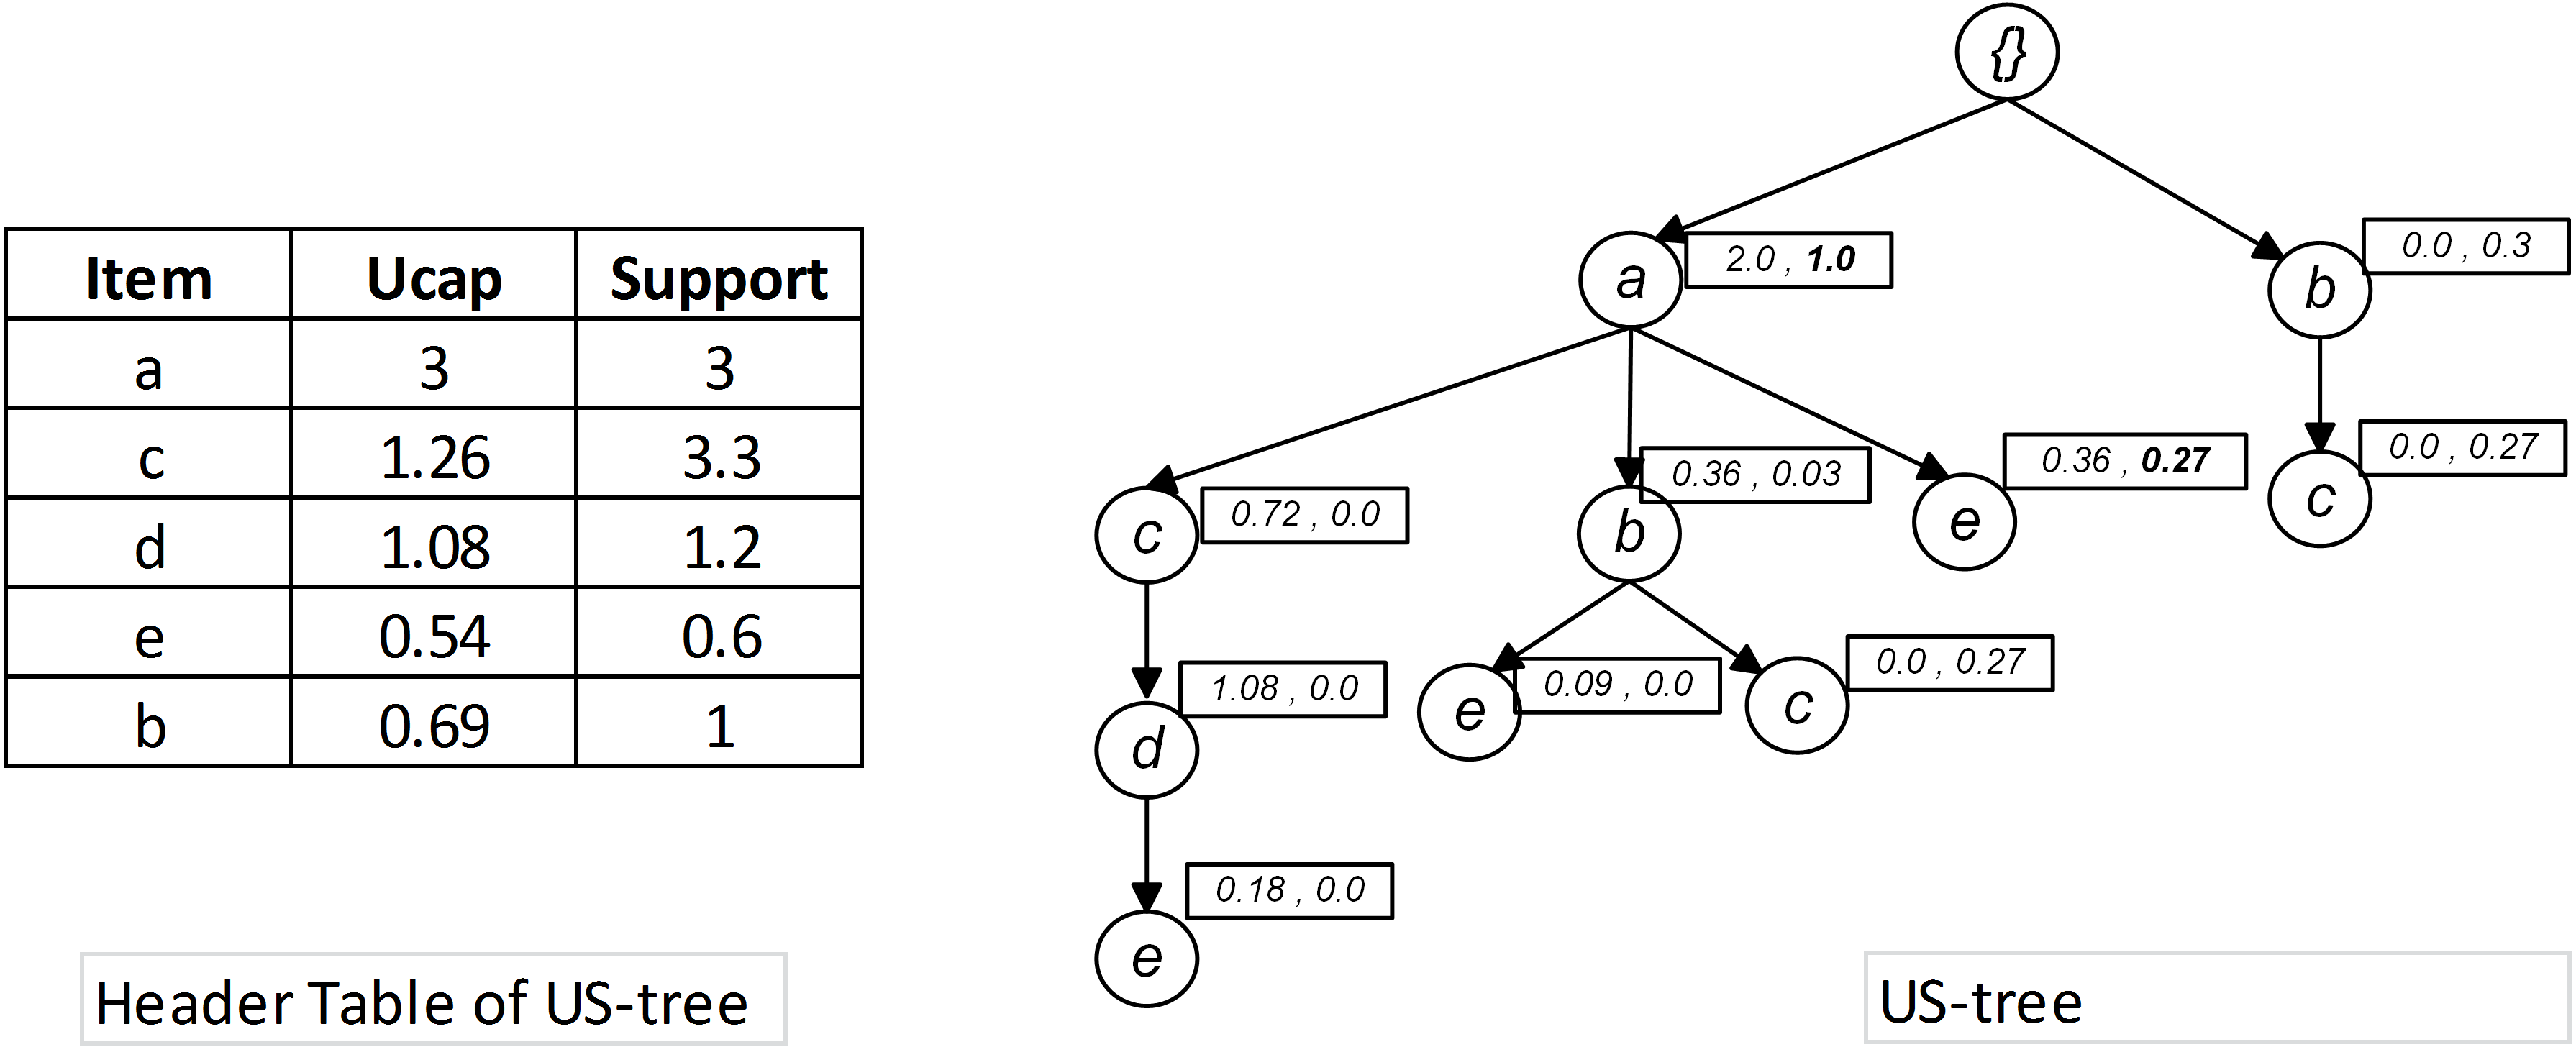
\includegraphics[width=0.9\textwidth]{visio/us_tree}  
	\caption{Snapshot of US-tree with Header Table}%%%%%%%%%%%%%%%
	\label{figure:US_TREE_HEADER_TABLE}
    \end{minipage}%
    \begin{minipage}{0.5\linewidth}
    \centering
%	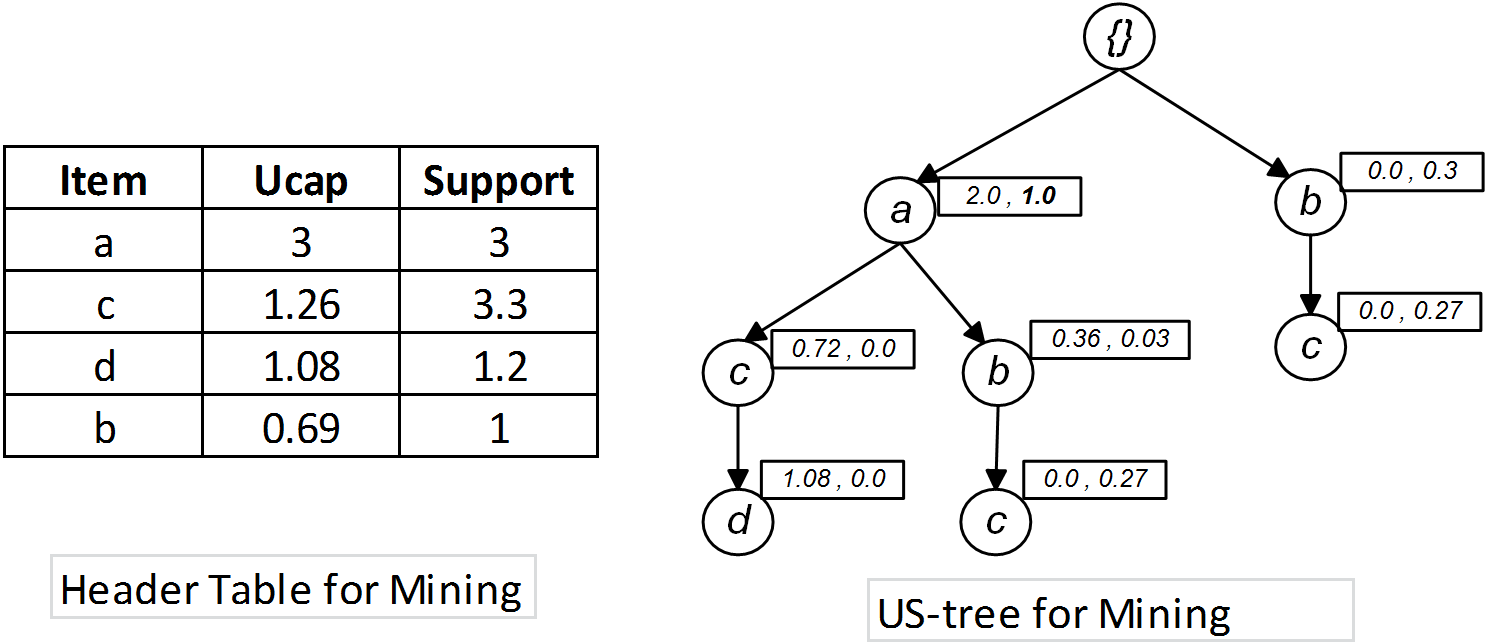
\includegraphics[width=0.9\textwidth]{visio/M_TREE}  
%	\caption{$e$-cond Tree and corresponding Header Table}%%%%%%%%%%%%%%%
%	\label{figure:E_COND_TREE_HEADER_TABLE}
%	
%	
		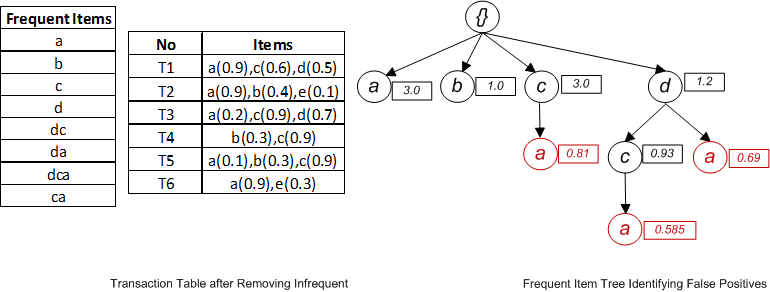
\includegraphics[width=0.9\textwidth]{visio/frequent_tree_final_ex}  
	\caption{Frequent Patterns, Transaction (non-frequent removed), Frequent Pattern-tree with False positives in red}%%%%%%%%%%%
	\label{figure:FALSE_NEGATIVE}
    \end{minipage}
\end{figure*}
%
%\begin{figure}[t]
%    \centering
%	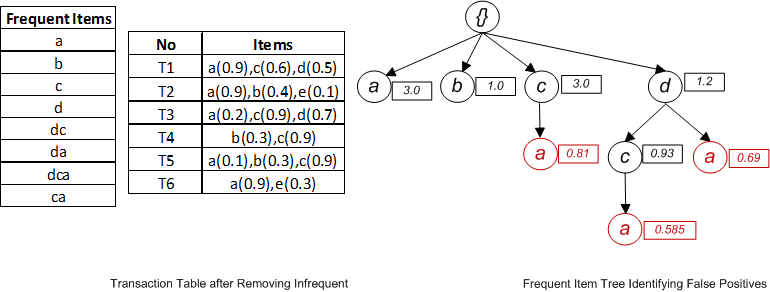
\includegraphics[width=0.5\textwidth]{visio/frequent_tree_final_ex}  
%	\caption{Frequent Patterns, Transaction (non-frequent removed), Frequent Pattern-tree with False positives in red}%%%%%%%%%%%%%%%
%	\label{figure:FALSE_NEGATIVE}
%\end{figure}

\subsubsection{US-tree Construction}
A batch of transactions need to be inserted into the tree in its own window slot. After inserting all batches, the window will be complete and be ready to mine. Previously, we claimed that our tree will be very compact. For this, we have proposed an approach for sharing nodes. To share same tree nodes, two items with same id and order should not care about own existential probability. If item is already in the tree with same id then two items should share the node. Thus the tree will be very compact. When inserting an item in the tree, the \emph{U\textsuperscript{cap}} of the tree should be updated by adding the prefix value of the node. Thus each batch should be inserted into the tree.

To construct tree for Table \ref{table:prefix_assigned}, first, we insert \emph{$Batch_{1}$ (T\textsubscript{1}, T\textsubscript{2}, T\textsubscript{3})} in the $Window_{1}$. To insert \emph{T\textsubscript{1} - a(0.9), c(0.54), d(0.45), e(0.18)}, we insert item \emph{$a$(0.9)} as a child of root \emph{\{\}}. Update $a$'s prefix value as $0.9$. Then we add \emph{$c$(0.54)} as $a$'s child and update $c$'s prefix value as $0.54$. Then, adding \emph{$d$(0.45)} as $c$'s child and update $d$'s prefix value as $0.45$. After that \emph{$e$(0.18)} is added as $d$'s child and update $e$'s prefix value as $0.18$. Hence, \emph{$T_{1}$} is inserted into the tree as shown in part 1 of Figure \ref{figure:t1_6}.

For \emph{T\textsubscript{2} - a(0.9), b(0.36), e(0.09)} first we insert \emph{$a$(0.9)}. Here we found \emph{$a$} is already inserted, so we just update existing node $a$'s prefix value $0.9 + 0.9 = 1.8$ (part 2 of Figure \ref{figure:t1_6}. Then we insert \emph{$b$(0.36)}. As \emph{$a$} has no child labeled \emph{$b$}, we insert a new child $b$ and update its prefix value to $0.36$. Then, we insert new $e$(0.09) as the child of \emph{$b$}. For \emph{T\textsubscript{3} - a(0.2), c(0.18), d(0.63)}, we follow the existing path \emph{a(1.8), c(0.54), d(0.45)} and update corresponding prefix value as $1.8 + 0.2 = 2.0$, $0.54 + 0.18 = 0.72$ and $0.45 + 0.63 = 1.08$ (part 3 of Figure \ref{figure:t1_6}. After inserting \emph{T\textsubscript{3}}, $Window_{1}$ is completed. Then we will go for inserting next batch \emph{$Batch_2$ (T\textsubscript{4}, T\textsubscript{5}, T\textsubscript{6})} in the tree. For \emph{$Batch_{2}$}, we shall put prefix value in the newest slots of the window. Thus, the latest batch becomes the most recent information container. For inserting \emph{T\textsubscript{4} - b(0.3), c(0.27)}, we insert new node \emph{$b$} as there is no child of $b$ of the root node \emph{\{\}}. So, we insert \emph{$b$} as a child of the root \emph{\{\}} node and update its prefix value to $0.3$. Then, we insert \emph{$c$(0.27)} as child of \emph{$b$} and update prefix value to $0.27$. As \emph{T\textsubscript{4}} belongs to \emph{$Batch_{4}$}, we update prefix value for recent batches. After that we insert \emph{T\textsubscript{5} - a(0.1), b(0.03), c(0.27)}. We merge \emph{a(0.1), b(0.03)} with previous \emph{a, b } nodes and update prefix value $0.1$ and $0.03$ in the slot of second batch. Finally, we insert new node \emph{$b$} as a child of \emph{$b$} and update its prefix value to $0.27$ (Figure \ref{figure:t1_6}.
    
Now our window is complete and we can start \emph{USFP-growth} mining in \emph {US-tree}. When new transactions and batches come, like \emph{$Batch_{3}$, i.e., (T\textsubscript{7}, T\textsubscript{8}, T\textsubscript{9})}, these need to be inserted into the tree by sliding the window. For this, when we construct the tree, we maintain a header table which contains the information for the oldest data. That is, pointer points to the oldest data and can be found easily to slide the whole tree. Figure-\ref{figure:t7_9} shows the sliding process, getting the tree with no old data and ready to insert next batch \emph{$Batch_{3}$}. After inserting \emph{$Batch_{3}$}, we get the tree like Figure-\ref{figure:t7_9}.
  
In the described \emph{US-tree} construction process, we see that tree sharing is very much common and regular. That makes our tree very compact and memory needed to hold items was significantly small. Moreover, the tree construction time improves surprisingly. As the tree size is small, less number of conditional trees will be generated and those will be smaller in volume. As a result those can be mined faster.

\subsubsection{FPUS-growth Mining Approach}
In this section we will discuss about our mining approach \emph{USFP-growth} to find frequent patterns. For mining, we used \emph{FP-growth} like approach. Generally, we can remove all the nodes having support less than \emph{minimum support}. From header table, we get which nodes is less than \emph{minimum support}. As we mentioned earlier, for \emph{U\textsuperscript{cap}} value, we took the upper limit, hence, we can remove all the nodes having prefix value less than \emph{minimum support}. In this process, we can eliminate most of the infrequent nodes from the tree. For this purpose, we used header table that was created during the creation of \emph{US-tree}. Then we construct conditional tree starting from the lowest support holding node. From header table, we also get the position of all nodes containing same item in the tree.

Figure-\ref{figure:US_TREE_HEADER_TABLE} shows \emph{US-Tree} for mining and corresponding header table before starting mining. From the header table, we get the support of \emph{a} = $3.00$, \emph{b} = $1.00$, \emph{c} = $3.30$, \emph{d} = $1.20$ and \emph{e} = $0.60$. So, \emph{$e$} is not frequent length 1 pattern. Hence, it is guaranteed that no item set containing \emph{e} will be frequent, due to the downward closure property of frequent item set. So we remove the node \emph{e} and get the new mining tree Figure-\ref{figure:E_COND_TREE_HEADER_TABLE} and its header table. Here we find all one item sets that are frequent, i.e., \emph{\{a\}, \{b\}, \{c\} \{d\}}. Now we will construct conditional tree for the found frequent 1-item and mine the conditional tree for it. However, items having total \emph{U\textsuperscript{cap}} less than \emph{minimum support} is not considered to construct conditional tree because this \emph{U\textsuperscript{cap}} value has been taken as the upper bound. So total \emph{U\textsuperscript{cap}} value less than \emph{minimum support} indicates that item must not be exist in the $2$ or more length frequent item set. So we do not construct conditional tree for these items.
% figure:FALSE_NEGATIVE figure:E_COND_TREE_HEADER_TABLE
We construct conditional trees from items having lowest total \emph{U\textsuperscript{cap}} value greater than \emph{minimum support}. As \emph{b} having total \emph{U\textsuperscript{cap}}, that is, $.69$, \emph{b} is skipped. Then the next candidate is \emph{d}. From header table pointer, we find that there is only one path for item \emph{d} exists in the mining tree (shown in Figure-\ref{figure:E_COND_TREE_HEADER_TABLE}), that is, \{\emph{a, c, d}\}:$1.08$. So we create conditional tree and update all nodes for mining probability with \emph{d's} \emph{U\textsuperscript{cap}} $1.08$. For this conditional tree, (Figure-\ref{figure:E_COND_TREE_HEADER_TABLE}) the header tables says all the nodes in the tree are having \emph{U\textsuperscript{cap}} greater than \emph{minimum support}, that is, $.9$. So, all the items are ready to be constructed as conditional tree. Since only one branch is found, we do not further construct conditional tree and take all the combinations as frequent items (Figure-\ref{figure:E_COND_TREE_HEADER_TABLE}. So we find \emph{\{dc\}, \{da\}, \{dca\}} as frequent pattern. 

Next we create conditional tree for \emph{c}. Here $c$ exists in the tree for three paths those are \emph{\{a, c\} : $0.72$ , \{a , b, c\} : $.027$ and \{b, c\} : $0.27$}. So we create conditional tree (Figure-\ref{figure:E_COND_TREE_HEADER_TABLE}). Total mining value of \emph{c} is the sum of item caps in each respective path of \emph{c}. From the header, we see that \emph{b} has total cap having less than \emph{minimum support}, so we remove \emph{b} and create two length item set \emph{\{ca\}}. Next, we construct \emph{ca} conditional tree that contains only root (\emph{\{\}}). So no further tree is needed to be constructed and mined. Than we create conditional tree for \emph{a}. We find only root \emph{\{\}} as prefix. This way, we get all the frequent patterns, i.e. \emph{\{a\}, \{b\}, \{c\} \{d\}, \{dc\}, \{da\}, \{dca\} and \{ca\}}. As we have found all patterns from the upper bound, it is guaranteed that there will be no false negatives. However, some false positives may exist in the found frequent item set as there may be some value less than maximum value we assumed. Then we go for false positive elimination.

\begin{figure*}[t]
    \begin{minipage}{0.25\linewidth}
        \centering
  		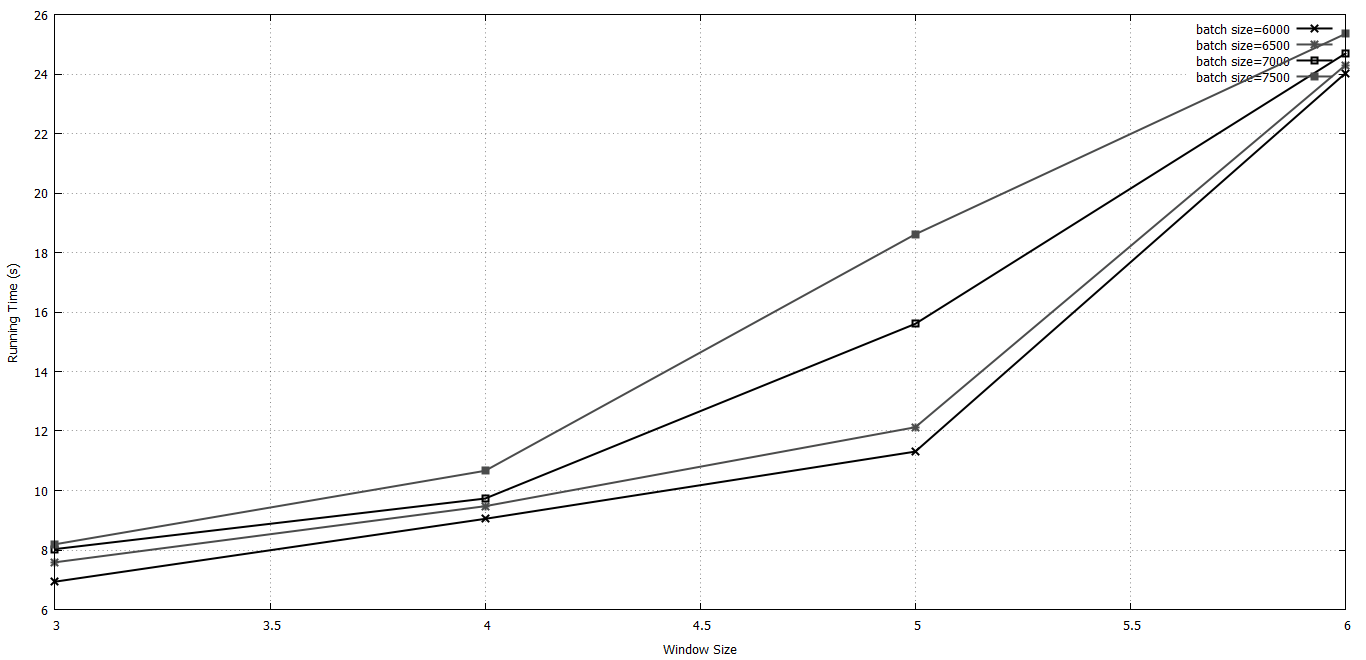
\includegraphics[width=\textwidth]{images/result/g_t10_const_batch}
  		\caption{T40I10D100K Dataset }
  		\label{result:g_t10_const_batch}
    \end{minipage}%	
    \begin{minipage}{0.25\linewidth}
         \centering
  		 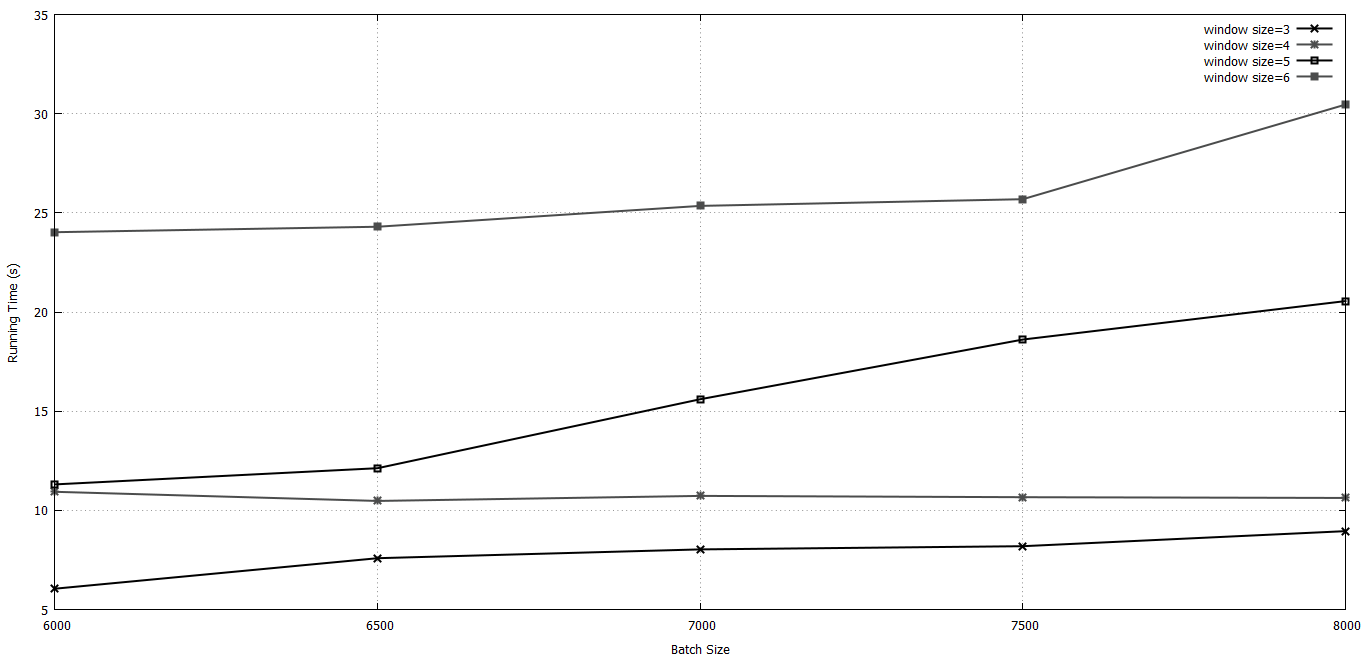
\includegraphics[width=\textwidth]{images/result/g_t10_const_win}
  		 \caption{ T40I10D100K Dataset }
  		 \label{result:g_t10_const_win}
    \end{minipage}	
	\begin{minipage}{0.25\linewidth}
		\centering
		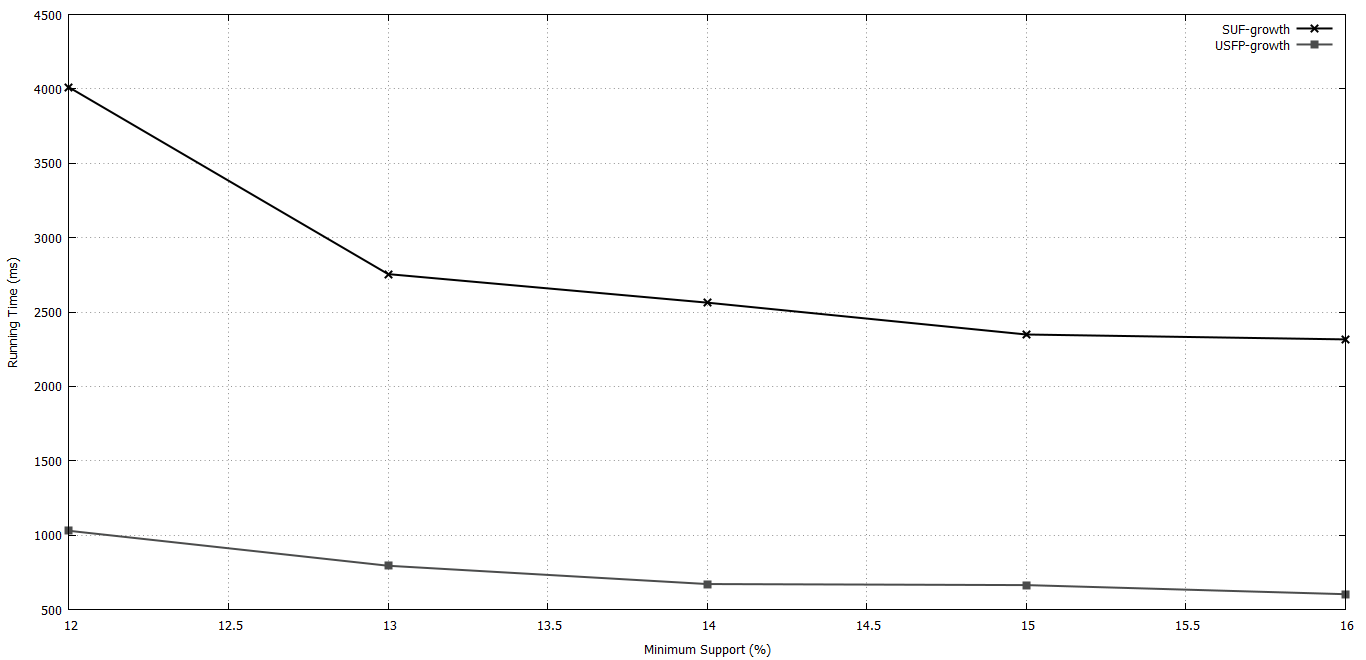
\includegraphics[width=\textwidth]{images/result/g_m_total}
		\caption{ Mushroom Dataset }
		\label{result:g_m_total}
	\end{minipage}%
    \begin{minipage}{0.25\linewidth}
		\centering
		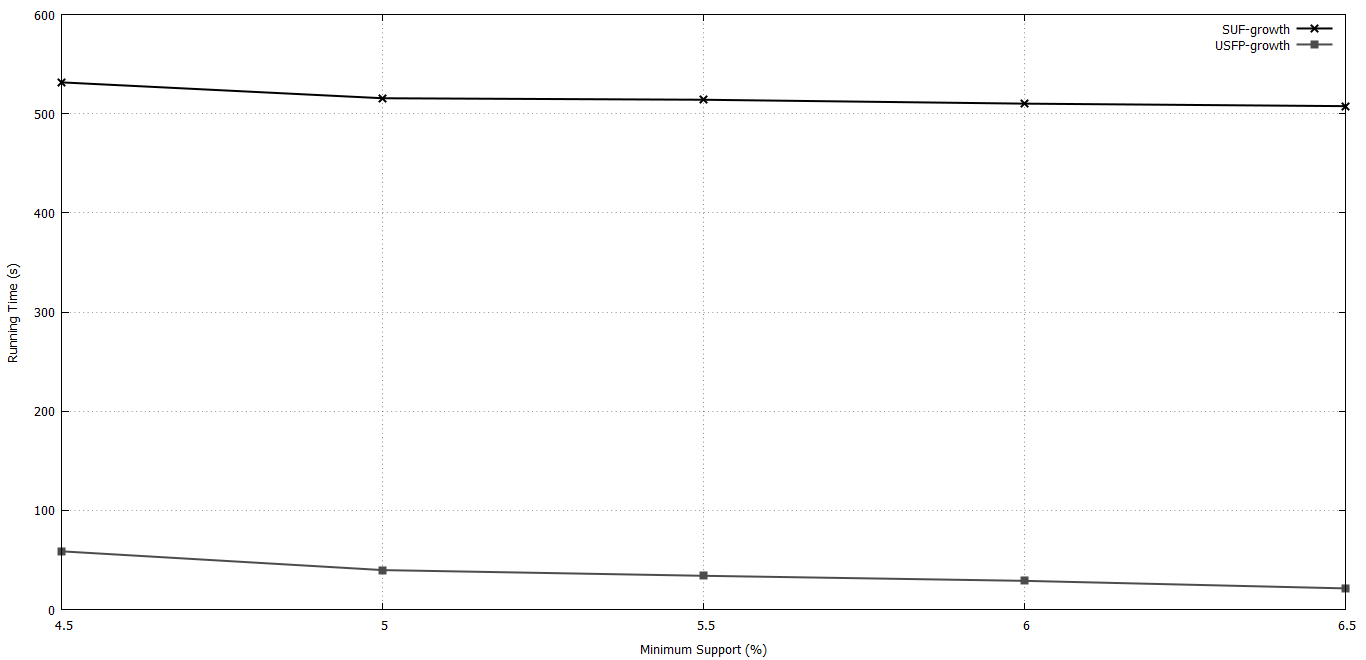
\includegraphics[width=\textwidth]{images/result/g_t10_total}
		\caption{ T40I10D100K Dataset }
		\label{result:g_t10_total}
    \end{minipage}	
\end{figure*}


\subsubsection{False positive reduction}
    To recall, false positives are such patterns those exist in the frequent pattern list but not actually frequent. False negatives are such patterns those do not exist in the frequent pattern list but actually frequent. In our approach, the process of \emph{U\textsuperscript{cap}} assignment, construction of \emph{US-tree} and \emph{USFP-growth} mining, all are based on taking upper value of two item set supports, this may generate some false positives but no false negatives. In this section, we will discuss about finding and eliminating all the false positives from generated patterns by \emph{USFP-growth} mining. For this elimination process, we just use two scans of transactions. In the first scan we eliminate the infrequent one item set and in the second scan, we update \emph{frequent tree} exact support that finds infrequent items if exists in our frequent found items. The process is given below. 

Mining on Table-\ref{table:prefix_assigned} generates \emph{\{a\}, \{b\}, \{c\} \{d\}, \{dc\}, \{da\}, \{dca\}} and \emph{\{ca\}} as frequent patterns. We need to construct a pattern tree from the patterns using the similar approach of constructing FP-tree in FP-growth algorithm.

%Mining on Table-\ref{table:prefix_assigned} generates \emph{\{a\}, \{b\}, \{c\} \{d\}, \{dc\}, \{da\}, \{dca\}} and \emph{\{ca\}} as frequent patterns. We need to construct a pattern tree from the patterns. For tree construction we first create root node \emph{\{\}}. Then take each frequent item and insert into the root node as a child. for \emph{a}, \emph{b}, \emph{c} and \emph{d} we just insert them as child of root node, since these do not exists in the tree. For \emph{dc}, no need to create new node for \emph{d} but create a new node \emph{c} as child of \emph{d} as there is no \emph{c} exists in the child of \emph{d}. Thus we construct the whole frequent pattern tree for further identification of infrequent patterns.

Next, in the first scan of inserted transactions, we remove all one length infrequent items from transactions. Figure-\ref{figure:FALSE_NEGATIVE} shows the transaction table after eliminating all nodes except one length frequent items. Since, for one length items, checking whether they are frequent, requires no upper bound limit and we get exact one length frequent patterns. From our \emph{Frequent Item Tree}, all the children of \emph{root \{\}} are frequent and there are no false positives, i.e., \emph{\{a\}, \{b\}, \{c\} \{d\}}. All other items are infrequent. Then in the second scan we take each transaction and update each nodes support. In the tree, we update value with the equation-\ref{equation:cap}. At the second scan, \emph{Frequent Item Tree} becomes complete with all information to find infrequent items in generated patterns. Now, we need to traverse the \emph{Frequent Item Tree}. As the tree contains all nodes with its own support we get the true infrequent. For example, for the path \emph{\{d, a\}}, \emph{a : 0.89} contains the actual support for the pattern {da : 0.89}. We find this in frequent, so we can easily eliminate this. Figure-\ref{figure:FALSE_NEGATIVE} depicts the infrequent patterns within frequent patterns. Therefore, we can eliminate all the false positives and find the exact frequent patterns. From the tree we find the patterns \emph{\{a\}, \{b\}, \{c\} \{d\} and \{dc\}} as exactly frequent.

%      \begin{figure}[]
        \centering
            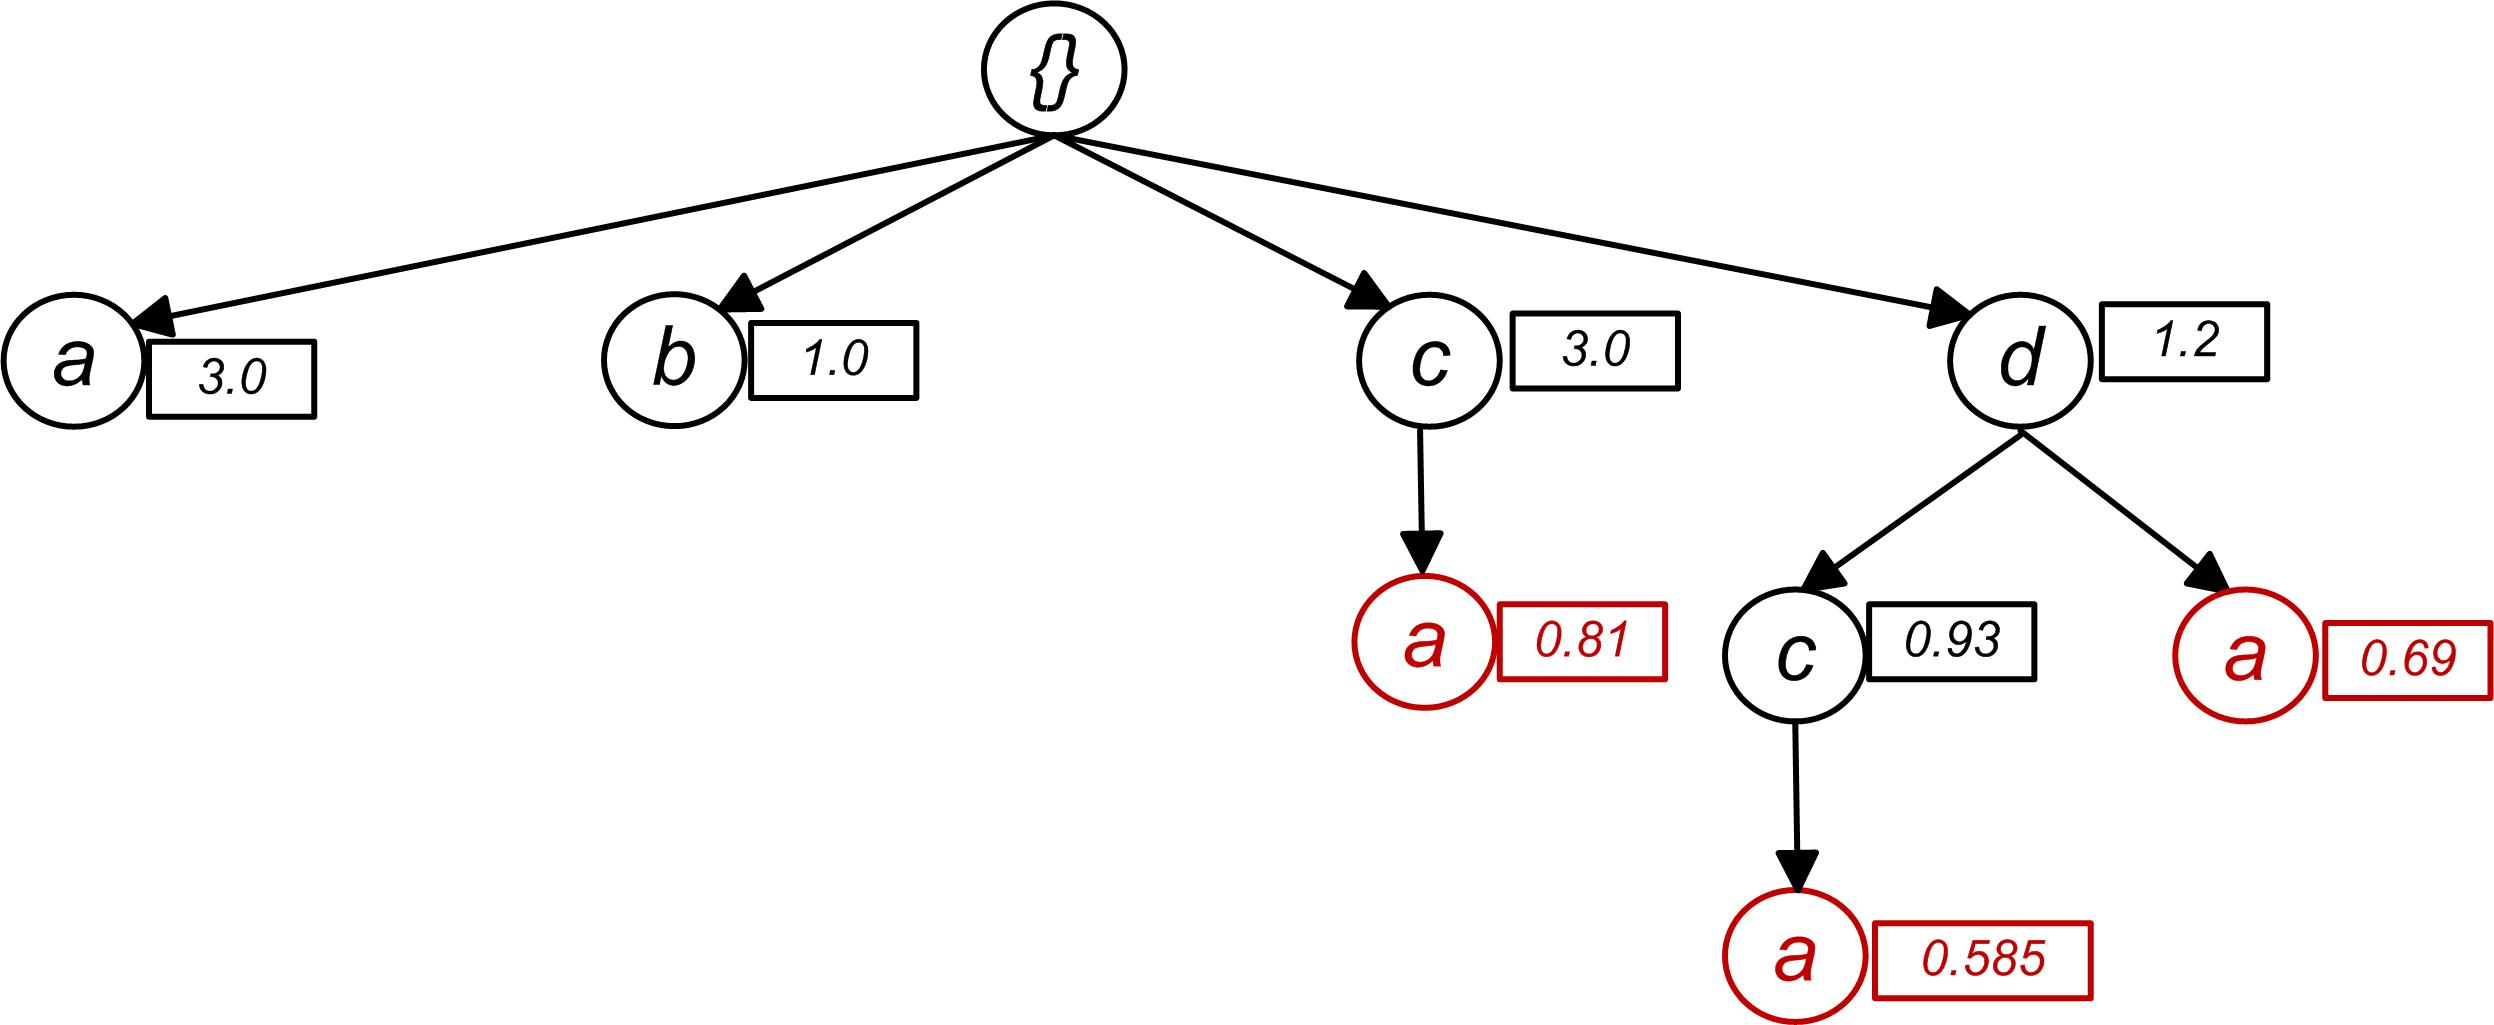
\includegraphics[width=.45\textwidth]{images/frequent_tree_final}
        \caption{Pattern Tree Identifying False Positives}
        \label{figure:frequent_patterns_final}
  \end{figure}



\begin{figure}
\begin{minipage}{0.15\textwidth}
  \centering
  
	\begin{center}
	\begin{tabular}{ |c| } 
 	\hline
 		FPs\\ \hline\hline
 		a \\ \hline
 		b \\ \hline
 		c \\ \hline
 		d \\ \hline
 		dc \\ \hline
 		da \\ \hline
 		dca \\ \hline
 		ca \\ \hline
\end{tabular}
\end{center}  


  \captionof{table}{Frequent Patterns}
\end{minipage}
\hfill
\begin{minipage}{0.30\textwidth}
  \centering
  
  \begin{center}
  \begin{tabular}{ |c|c| } 
  \hline
    No & Items \\ \hline\hline
    T\textsubscript{1} & \emph{a(0.9),c(0.6),d(0.5)}\\ \hline
    T\textsubscript{2}& \emph{a(0.9),b(0.4),e(0.1)}\\ \hline
    T\textsubscript{3}& \emph{a(0.2),c(0.9),d(0.7)}\\ \hline
    T\textsubscript{4}& \emph{b(0.3),c(0.9)}\\ \hline
    T\textsubscript{5}& \emph{a(0.1),b(0.3),c(0.9)} \\ \hline
    T\textsubscript{6} & \emph{a(0.9),e(0.3)
}\\ \hline
\end{tabular}
\end{center}  
  \captionof{table}{Transaction Table after Removing Infrequent}


\end{minipage}
\label{figure:frequent_patterns}
\end{figure}


\begin{figure*}[t]
\begin{minipage}{0.25\linewidth}
    \centering
    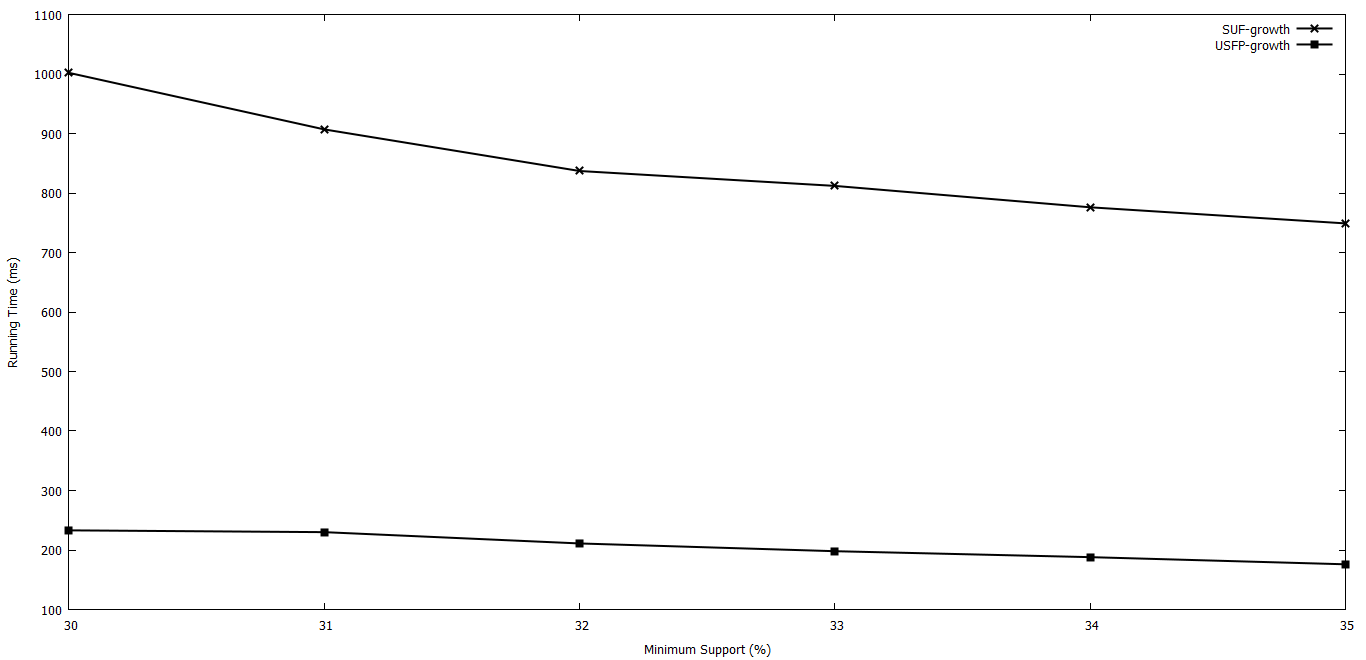
\includegraphics[width=\textwidth]{images/result/g_chess_total}
    \caption{Chess Dataset }
    \label{result:g_chess_total}
\end{minipage}%
\begin{minipage}{0.25\linewidth}
   \centering
   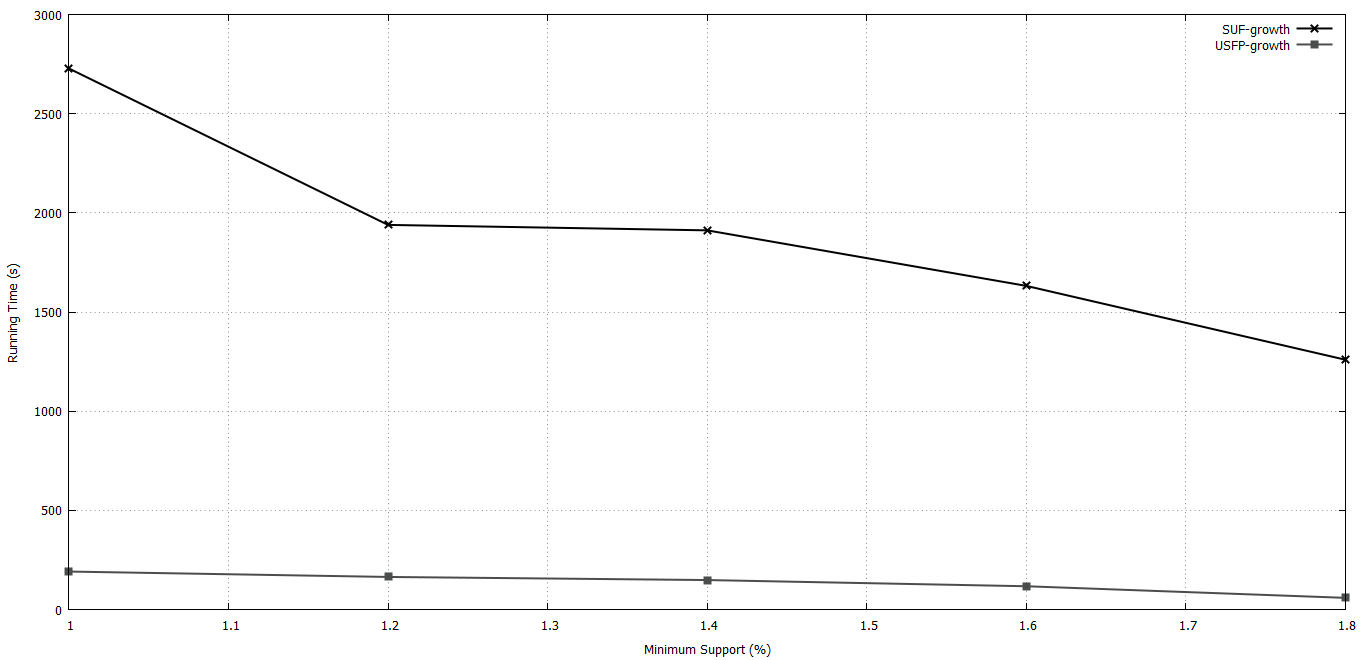
\includegraphics[width=\textwidth]{images/result/g_k_total}
   \caption{Kosarak Dataset }
   \label{result:g_k_total}
    \end{minipage}
\begin{minipage}{0.25\linewidth}
    \centering
    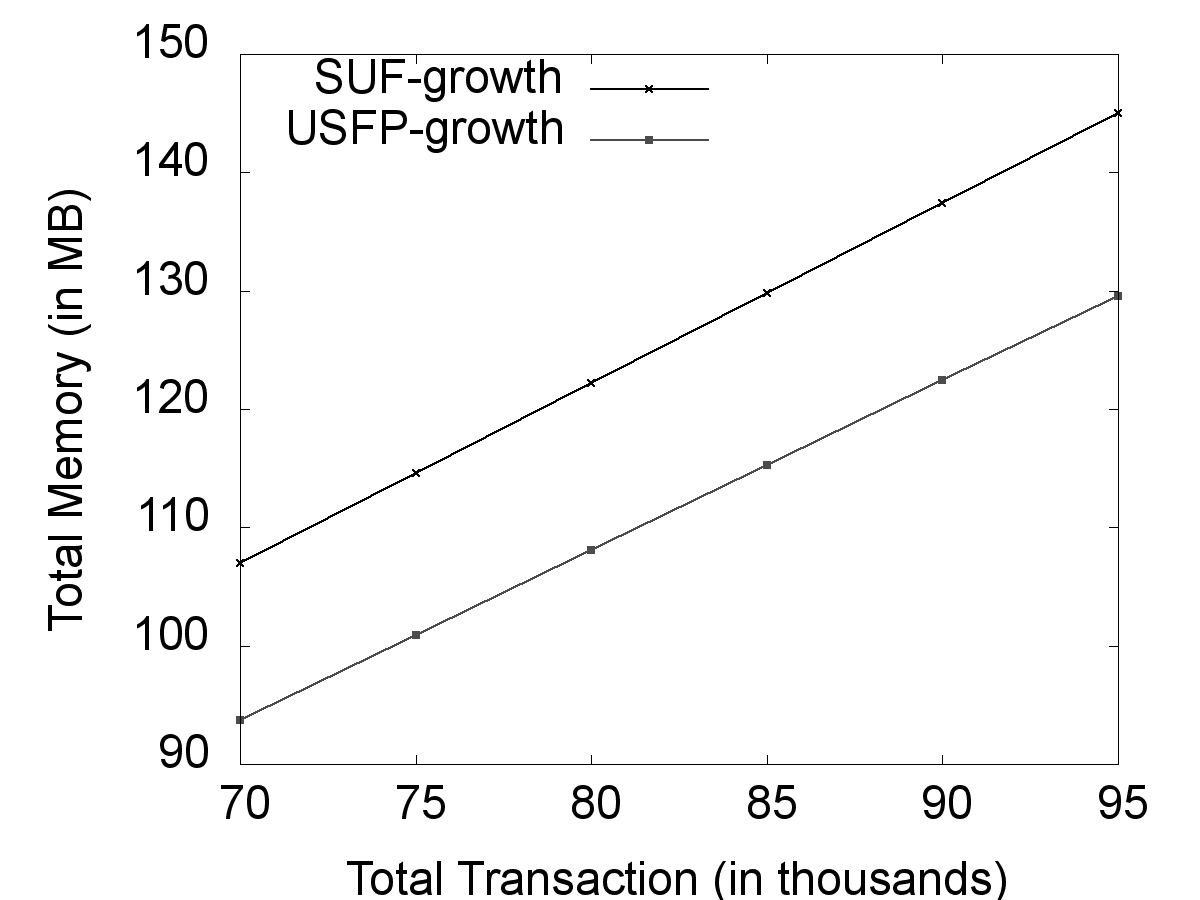
\includegraphics[width=\textwidth]{images/result/g_t10_memory_node}
    \caption{T40I10D100K Dataset }
    \label{result:g_t10_memory_node}
\end{minipage}%
\begin{minipage}{0.25\linewidth}
   \centering
   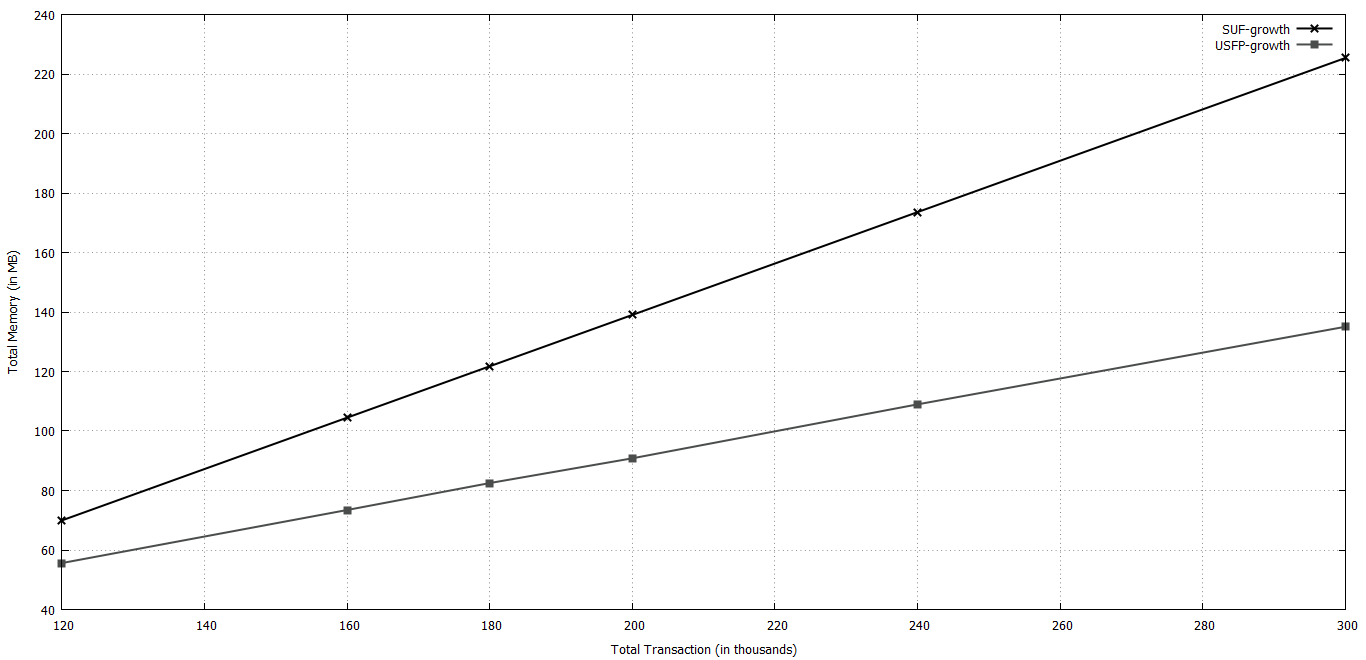
\includegraphics[width=\textwidth]{images/result/g_k_memory_node}
   \caption{Kosarak Dataset }
   \label{result:g_k_memory_node}
    \end{minipage}
\end{figure*}

\section{Experimental Results}\label{Experiment}
We have performed a number of simulations in our experiment on both synthetic database and real-world database. The data are taken from dataset repository ~\cite{dataset}. Performance tests from our experiment show that \emph{US-tree} tree construction technique and \emph{USFP-growth} mining algorithm can run on any uncertain stream database with any support threshold, window size, and batch size. Our experimental result shows that these techniques are much faster and scalable frequent pattern mining technique. We have tried to compare in all aspects to prove our approach's scalability, run-time efficiency and memory efficiency.  

For experimentation, we collected data from dataset repository ~\cite{dataset} which contain precise (certain) data. Then we have used our own probabilistic tool and technique to generate the existential probability of each item of the each transaction of the database. Real life data set actually follows gaussian distribution that is normal distribution. It actually says that in real world extreme cases are minimum and average cases are maximum. We have used \emph{Java pseudo random} to generate the existential probability for each item of all the transaction of the database with gaussian distribution. By assigning these probability value to each item, we have generated the uncertain database for both real life database and synthetic database. 

However, one can give existential probability by any distribution according to need. We have set several parameters for the evaluation like batch size vs running time, window size vs running time, transactions in a window vs false positive count for correctness; tree construction time per window and total database vs minimum support, mining time per window and total database vs minimum support, total time to complete per window and total database vs minimum support, total tree node in tree per window vs minimum support, total memory needed by mining process vs minimum support for comparison with existing approaches.

For the extensive experimental analysis, we have chosen the mushroom, chess and T40I10D100K datasets. The reason we have chosen these two datasets is, the mushroom  is real life dataset and dense dataset whereas T40I10D100K  is synthetic and sparse dataset generated by a generator from the IBM Almaden Quest.
\subsection{Performance Analysis}

\paragraph{Window Size Change Effect}For window size change effect we have assessed our algorithm in the different angle. The experiment shows that the varying window size doesn't affects the performance and it is consistent w.r.t. runtime (including tree construction, mining, and false positive reduction). Figure \ref{result:g_t10_const_batch} shows the effect of different window size for T40I10D100K dataset on runtime.
                
\paragraph{Batch Size Change Effect}We have also tested the performance of our algorithm by changing the batch size. For varying batch size in different volume, the result was consistent. For constant window and variable batches we have simulated our proposed algorithms. Figure-\ref{result:g_t10_const_win} shows effect of batch size change effect on T40I10D100K dataset. 
        
\subsection{Performance Comparison With Existing Approaches}
In this section, we have compared our proposed approach with existing algorithm. We have chosen SUF-growth ~\cite{DBLP:conf/icde/LeungH09} (most recent, latest state-of-the-arts algorithm) for comparison. This fits perfectly for uncertain stream data mining. UF-streaming also designed for mining frequent patterns from uncertain stream but in ~\cite{DBLP:conf/icde/LeungH09} it has been proved that in all criteria (runtime, memory and correctness) SUF-growth ~\cite{DBLP:conf/icde/LeungH09} is better than UF-streaming ~\cite{DBLP:conf/icde/LeungH09}.
            
\subsubsection{Runtime Comparison}
Our proposed approach has been assessed based on runtime against existing algorithm using both dense and sparse datasets. For mushroom dataset, total processing and running time of proposed algorithm have been compared with SUF-growth ~\cite{DBLP:conf/icde/LeungH09} algorithm running time. Figure-\ref{result:g_m_total} shows the result graph. As mushroom is a dense database we noticed significant gain. For dense characteristics, the constructed \emph{US-tree} is very much compact and moreover when mining compact tree, the mining time surprisingly decreases that affect the total time. Figure-\ref{result:g_t10_total} shows same comparison for T40I10D100K dataset. The graphs show that our algorithm works correctly for sparse dataset too. Figure-\ref{result:g_chess_total} shows running time for chess dataset. Kosarak is very large and real-life web-click data set. This database is sparse and very much large. Figure-\ref{result:g_k_total} shows the superiority of our proposed algorithm w.r.t. running time for varying thresholds.
       
\subsubsection{Memory Comparison}
As our proposed \emph{US-tree} have the capability to share nodes more than \emph{SUF-growth}, we get much more gain in memory. The experimental result comply the fact. Figure-\ref{result:g_t10_memory_node} and Figure \ref{result:g_k_memory_node} show the memory comparison on T40I10D100K and Kosarak datasets. The graph clearly shows that with the increase of total transaction in the tree gives the much more gain. On these sparse databases, it has been clearly shown that lot of memory optimization has been possible with our proposed algorithm. As the database is sparse, we get the memory gain less than dense one.

In summary, our proposed \emph{US-tree} construction \emph{USFP-growth} mining approach is correct, efficient, scalable and works fine in any configuration (minimum support, window size, batch size). For dense dataset (both real and synthetic) our approach is very efficient. For sparse dataset, this also gives us gain both in memory and running time. The \emph{U\textsuperscript{cap}} value gives much more benefit to share nodes in the \emph{US-tree}. The compactness of \emph{US-tree} is noticeable. Mining compact \emph{US-tree} gives the main surprise in the running time. The \emph{USFP-growth} mining algorithm works nicely without generating any false negatives and a little amount of false positives that can efficiently be removed using the false positive reduction technique.

\section{Conclusions}\label{Conclusion}
In this paper, we have proposed new sliding window based probabilistic strategy for finding frequent patterns from uncertain dynamic data. The strategy comprises of a new upper bound of existential probability, \emph{U\textsuperscript{cap}}, a new compact data-structure, \emph{US-tree} and an efficient algorithm \emph{USFP-growth} that recursively mine frequent patterns from \emph{US-tree}. For calculating \emph{U\textsuperscript{cap}} value, we have taken upper-bound of existential probability that makes the node sharing possible between same items. For uncertainty property of data, node sharing was very much irregular in existing approaches. In our strategy, node sharing is possible more frequently and this makes the tree more compact and efficient. To handle the stream of data, we have segmented the whole transactions into batches and windows. Instead of keeping the support we have kept new meta-information based on \emph{U\textsuperscript{cap}} value that helps further mining. Our developed \emph{USFP-growth} mining algorithm efficiently removes unnecessary patterns from the tree earlier, which helps to improve runtime efficiency. We have also introduced an efficient strategy to remove the false positives generated by our algorithm. Our comprehensive experimental analyses proves the supremacy of proposed algorithm w.r.t. running time (efficiency), memory consumption (scalability). We also developed a frequent pattern tree which may later be used to mine closed patterns and maximal patterns.

\bibliographystyle{IEEEtran}
%\bibliography{mybib}
\bibliography{small_bibliography}

% that's all folks
\end{document}

